\documentclass[MASTER-SPC.tex]{subfiles}
\begin{document}
\section{Quality Control Charts (MA4605 Only)}
%Quality Control Charts
\begin{itemize}
\item In the Lab classes, we will look at using the R package qcc, which stands for quality
control charts. 
\item This package can be used to create the following.
Shewhart quality control charts for continuous, attribute and count data.
\begin{enumerate}
\item CUSUM and EWMA charts.
\item Operating characteristic curves.
\item Process capability analysis.
\item Pareto chart and cause-and-effect chart.
\item Multivariate control charts
\end{enumerate}
(We won’t have time to get through all of this material)
\item There are two inbuilt data sets, available from the qcc package, that we will use
\begin{enumerate}
\item pistonrings
\item orangejuice
\end{enumerate}

The “pistonrings” data set (diameter)
The first data set describes piston rings for an automotive engine are produced by a
forging process.
\item The inside diameter of the rings manufactured by the process is measured on 25
samples, each of size 5, drawn from a process being considered 'in control'.
There are further 15 sets of observation ( i.e. 40 batches in total) to demonstrate
alternate outcomes.
The dataset is restructured as a data set called “diameter”.
The “orangejuice” data set
The second data set describes frozen orange juice concentrate is packed in 6-oz
cardboard cans. These cans are formed on a machine by spinning them from
cardboard stock and attaching a metal bottom panel.
\end{itemize} 
%================================================ %
\section{More on Control Charts}

\subsection{Control Chart Selection}
\begin{itemize}
	\item Correct control chart selection is a critical part of creating a control chart. If the wrong control chart is selected, the control limits will not be correct for the data. 
	\item The type of control chart required is determined by the type of data to be plotted and the format in which it is collected. \item Data collected is either in variables or attributes format, and the amount of data contained in each sample (subgroup) collected is specified.
	
	\item \textbf{Variables data} is defined as a measurement such as height, weight, time, or length. Monetary values are also variables data. 
	\begin{itemize}
		\item[$\ast$] Generally, a measuring device such as a weighing scale, vernier, or clock produces this data. \item[$\ast$] Another characteristic of variables data is that it can contain decimal places e.g. 3.4, 8.2.
	\end{itemize}
	
	\item \textbf{Attributes data} is defined as a count such as the number of employees, the number of errors, the number of defective products, or the number of phone calls. A standard is set, and then an assessment is made to establish if the standard has been met. 
	\begin{itemize}
		\item[$\ast$] The number of times the standard is either met or not is the count. Attributes data never contains decimal places when it is collected, it is always whole numbers, e.g. 2, 15.
	\end{itemize}
\end{itemize}

%------------------------------------------------------------- %
\newpage

\subsection{Attribute Control Charts}

\begin{itemize}
	\item The Shewhart control chart plots quality characteristics that can be measured and expressed numerically. We measure weight, height, position, thickness, etc. If we cannot represent a particular quality characteristic numerically, or if it is impractical to do so, we then often resort to using a quality characteristic to sort or classify an item that is inspected into one of two "buckets".
	\item  An example of a common quality characteristic classification would be designating units as "conforming units" or "nonconforming units". 
	\item Another quality characteristic criteria would be sorting units into "non defective" and "defective" categories. Quality characteristics of that type are called \textit{\textbf{attributes}}.
	
	\item \textit{Note that there is a difference between "nonconforming to an engineering specification" and "defective" -- a nonconforming unit may function just fine and be, in fact, not defective at all, while a part can be "in spec" and not fucntion as desired (i.e., be defective).}
	
	\item Examples of quality characteristics that are attributes are the number of failures in a production run, the proportion of malfunctioning wafers in a lot, the number of people eating in the cafeteria on a given day, etc.
\end{itemize}
\subsection{Types of Attributes Control Charts}

\begin{itemize}
	\item Control charts dealing with the proportion or fraction of defective product are called  \textbf{\textit{p-charts}} (for proportion).
	\item Control charts dealing with the number of defective product are called  \textbf{\textit{np-charts}}.
	\item Control charts dealing with the number of defects or nonconformities are called \textbf{\textit{c-charts}} (for count).
	\item There is another chart which handles defects per unit, called the \textbf{\textit{u-chart}} (for unit). This applies when we wish to work with the average number of nonconformities per unit of product.
\end{itemize}

\newpage
\subsection{p-charts}
\begin{itemize}
	\item The p-chart is a type of control chart used to monitor the \textbf{proportion of nonconforming units} in a sample, where the sample proportion nonconforming is defined as the ratio of the number of nonconforming units to the sample size, n.
	\item The p-chart only accommodates dichotomous PASS/FAIL-type inspection as determined by a series of tests, effectively applying the specifications to the data before they are plotted on the chart. 
	\item Other types of control charts display the magnitude of the quality characteristic under study, making troubleshooting possible directly from those charts.
	\item A p-chart is an attributes control chart used with data collected in subgroups of varying sizes. Because the subgroup size can vary, it shows a proportion on nonconforming items rather than the actual count. 
	\textit{\item p-charts show how the process changes over time. The process attribute (or characteristic) is always described in a yes/no, pass/fail, go/no go form. }
	\item Example: use a p-chart to plot the proportion of incomplete insurance claim forms received weekly. The subgroup would vary, depending on the total number of claims each week. 
	%\item P-charts are used to determine if the process is stable and predictable, as well as to monitor the effects of process improvement theories.
\end{itemize}
\newpage
\subsection{np-charts}
The np-chart is a type of control chart used to monitor the number of nonconforming units in a sample. An np-chart is an \textit{attributes} control chart used with data collected in subgroups that are the \textbf{same size}. 
\newline
\newline
\noindent It is an adaptation of the p-chart and used in situations where personnel find it easier to interpret process performance in terms of concrete numbers of units rather than the somewhat more abstract proportion.
\newline
\newline
\noindent The np-chart differs from the p-chart in only the three following aspects:
\begin{itemize}
	\item The control limits are 
	\[n\bar p \pm 3\sqrt{n\bar p(1-\bar p)}\], where n is the sample size and $\bar{p}$ is the estimate of the long-term process mean established during control-chart setup.
	
	\item The number nonconforming (np), rather than the fraction nonconforming (p), is plotted against the control limits.
	
	\item The sample size, n, is constant.
\end{itemize}
%
%\subsubsection{Similarities and Differences}
%Both p-charts and np-charts show how the process, measured by the number of nonconforming items it produces, changes over time. The process attribute (or characteristic) is always described in a binary form (i.e. yes/no, pass/fail etc). 
%
%For example, the number of incomplete accident reports in a constant daily sample of five would be plotted on an np-chart. Np-charts are used to determine if the process is stable and predictable, as well as to monitor the effects of process improvement theories. 
%
%The np-chart shows the number of nonconforming units in subgroups of set sizes.

%EDIT - MOVE ALL REMAINING TEXT IN SECTION TO "ATTRIBUTES DATA"
%\subsection{When is it used?}
%
%Use np-charts when exploring the following:
%
%\begin{itemize}
%\item Do you need to assess system stability?
%
%\item Is the data the number of nonconforming items per subgroup?
%
%\item Are the subgroups the same size?
%
%\item Are there only two outcomes to any given check?
%
%\item Is the time order of subgroups preserved?
%\end{itemize}

%\subsection{Optimized Usage}
%Collect as many subgroups as possible before calculating control limits. With smaller amounts of data, the np-chart may not represent variability of the entire system. The more subgroups you use in control limit calculations, the more reliable the analysis will be. Typically, 20 to 25 subgroups will be used in control limit calculations.

%\subsection{Applications of np-charts}
%There are several applications for np-charts. When you begin improving a system, use them to assess the system’s stability .
%
%\noindent \textbf{Stratification:} After the stability has been assessed, determine if you need to stratify the data. You may find entirely different results between shifts, among workers, among different machines, among lots of materials, etc. To see if variability on the np-chart is caused by these factors, collect and enter data in a way that lets you stratify by time, location, symptom, operator, and lots.
%
%You can also use np-charts to analyze the results of process improvements. Here you would consider how the process is running and compare it to how it ran in the past. Are there fewer nonconforming units?
%
%Finally, use np-charts for standardization. This means you should continue collecting and analyzing data throughout the process operation. If you made changes to the system and stopped collecting data, you would have only perception and opinion to tell you whether the changes actually improved the system. Without a control chart, there is no way to know if the process has changed or to identify sources of process variability.
%--------------------------------------------------------------- %
\newpage
\subsection{The c-chart}



\begin{itemize}
	\item In this chart, we plot the number of defectives (per batch, per day, per machine, per 100 feet of pipe, etc.). 
	\item This chart assumes that defects of the quality attribute are rare, and the control limits in this chart are computed based on the Poisson distribution (distribution of rare events).
	
	\item The c-chart is a type of control chart used to monitor "count"-type data, typically total number of nonconformities per unit.It is also occasionally used to monitor the total number of events occurring in a given unit of time.
	
	\item The c-chart differs from the p-chart in that it accounts for the possibility of more than one nonconformity per inspection unit, and that (unlike the p-chart and u-chart) it requires a fixed sample size. 
	
	\item The p-chart models "pass"/"fail"-type inspection only, while the c-chart (and u-chart) give the ability to distinguish between (for example) 2 items which fail inspection because of one fault each and the same two items failing inspection with 5 faults each; in the former case, the p-chart will show two non-conformant items, while the c-chart will show 10 faults.
	
	\item The Poisson distribution is the basis for the chart and requires the following assumptions:
	\begin{itemize}
		\item[$\ast$] The number of opportunities or potential locations for nonconformities is very large
		\item[$\ast$] The probability of nonconformity at any location is small and constant
		\item[$\ast$] The inspection procedure is same for each sample and is carried out consistently from sample to sample
	\end{itemize}
\end{itemize}
%-------------------------------------------------------------- %
\newpage
\subsection{The u-chart}
\begin{itemize}
	\item In this chart we plot the rate of defectives, that is, the number of defectives divided by the number of units inspected (the n; e.g., feet of pipe, number of batches). 
	\item Unlike the C chart, this chart does not require a constant number of units, and it can be used, for example, when the batches (samples) are of different sizes.
	
	\item The u-chart is a type of control chart used to monitor "count"-type data where the sample size is greater than one, typically the average number of nonconformities per unit.
	
	\item The u-chart differs from the c-chart in that it accounts for the possibility that the number or size of inspection units for which nonconformities are to be counted may vary. Larger samples may be an economic necessity or may be necessary to increase the area of opportunity in order to track very low nonconformity levels.
\end{itemize}


%------------------------------------------- %
\section{Control Charts with the qcc Package}
\newpage
{
	\large
	\begin{framed}
		\begin{verbatim}
		# install.package(qcc)
		library(qcc)
		
		# series of value w/ mean of 10 with a little random noise added in
		x <- rep(10, 100) + rnorm(100)
		
		# a test series w/ a mean of 11
		new.x <- rep(11, 15) + rnorm(15)
		
		# qcc will flag the new points
		qcc(x, newdata=new.x, type="xbar.one")
		\end{verbatim}
	\end{framed}
}
% END OF PAGE 1
% GOOD SO FAR 



\begin{figure}[h!]
	\centering
	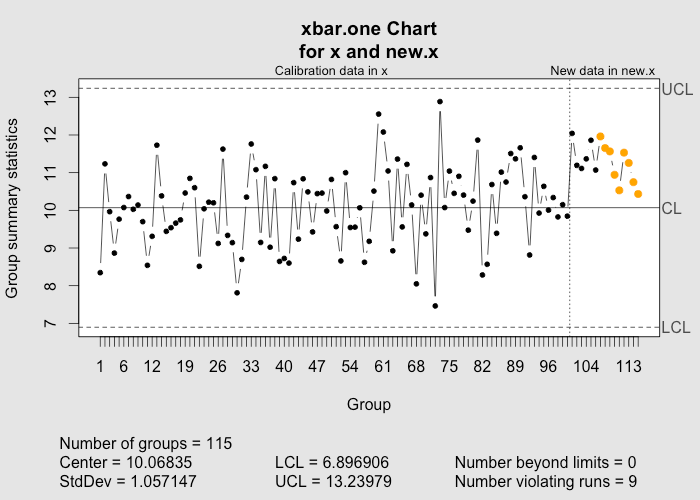
\includegraphics[width=0.9\linewidth]{./qcc-yhatexample}
	\caption{}
	\label{fig:qcc-yhatexample}
\end{figure}
\bigskip
\newpage
%-------------------------------------------- %
\begin{figure}[h!]
	\centering
	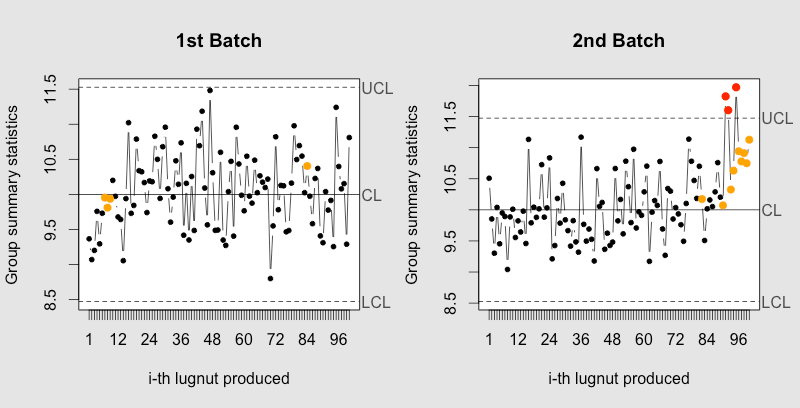
\includegraphics[width=0.90\linewidth]{./qcc_lugnuts1}
	
	\label{fig:qcc_lugnuts1}
\end{figure}
\begin{framed}
	\begin{verbatim}
	library(qcc)
	#make 2 plots in 1 figure
	par(mfrow=c(1,2))
	
	#points have base value of 10 w/ normally distributed error
	lugnuts <- rep(10, 100) + rnorm(100, mean=0, sd=0.5)
	qcc(lugnuts, type="xbar.one", center=10, add.stats=FALSE,
	title="1st Batch", 
	xlab="i-th lugnut produced")
	\end{verbatim}
\end{framed} 
\newpage
{
	\large
	\textbf{Second Batch }
	\begin{itemize}
		\item First 90 points have mean value of 10 with normally distributed error,
		\item Last 10 points have mean value of 11 with normally distributed error
	\end{itemize}
}
\begin{framed}
	\begin{verbatim}
	lugnuts <- c(rep(10, 90), rep(11, 10)) + rnorm(100, mean=0, sd=0.5)
	qcc(lugnuts, type="xbar.one", center=10, add.stats=FALSE,
	title="2nd Batch", 
	xlab="i-th lugnut produced")
	
	\end{verbatim}
\end{framed}
\newpage 

\begin{verbatim}
> set.seed(1234)
> lugnuts <- rep(10, 100) + rnorm(100, mean=0, sd=0.5)
> summary(lugnuts)
Min. 1st Qu.  Median    Mean 3rd Qu.    Max. 
8.827   9.552   9.808   9.922  10.240  11.270 
> length(lugnuts)
[1] 100
> newLugnuts <- rep(11, 10) + rnorm(10, mean=0, sd=0.5)
> summary(newLugnuts)
Min. 1st Qu.  Median    Mean 3rd Qu.    Max. 
10.55   10.75   11.00   10.92   11.08   11.21 
> length(newLugnuts)
[1] 10
\end{verbatim}

\begin{framed}
	\begin{verbatim}
	qcc1 <- qcc(lugnuts, type="xbar.one", center=10, add.stats=TRUE,
	title="1st Batch of 100", 
	xlab="i-th lugnut produced")
	
	
	
	qcc2 <- qcc(lugnuts, newdata=newLugnuts,
	type="xbar.one", center=10, 
	add.stats=TRUE, title="All Lugnuts", 
	xlab="i-th lugnut produced")
	
	mode(qcc1)
	class(qcc1)
	names(qcc1)
	\end{verbatim}
\end{framed}

\begin{verbatim}
> mode(qcc1)
[1] "list"
> class(qcc1)
[1] "qcc"
> names(qcc1)
[1] "call"       "type"       "data.name"  "data"       "statistics"
[6] "sizes"      "center"     "std.dev"    "nsigmas"    "limits"    
[11] "violations"
> qcc1$violations
$beyond.limits
integer(0)

$violating.runs
[1] 13 38 39 40 48 49 50 51 52 53 54 55
\end{verbatim}

\newpage
\begin{figure}[h!]
	\centering
	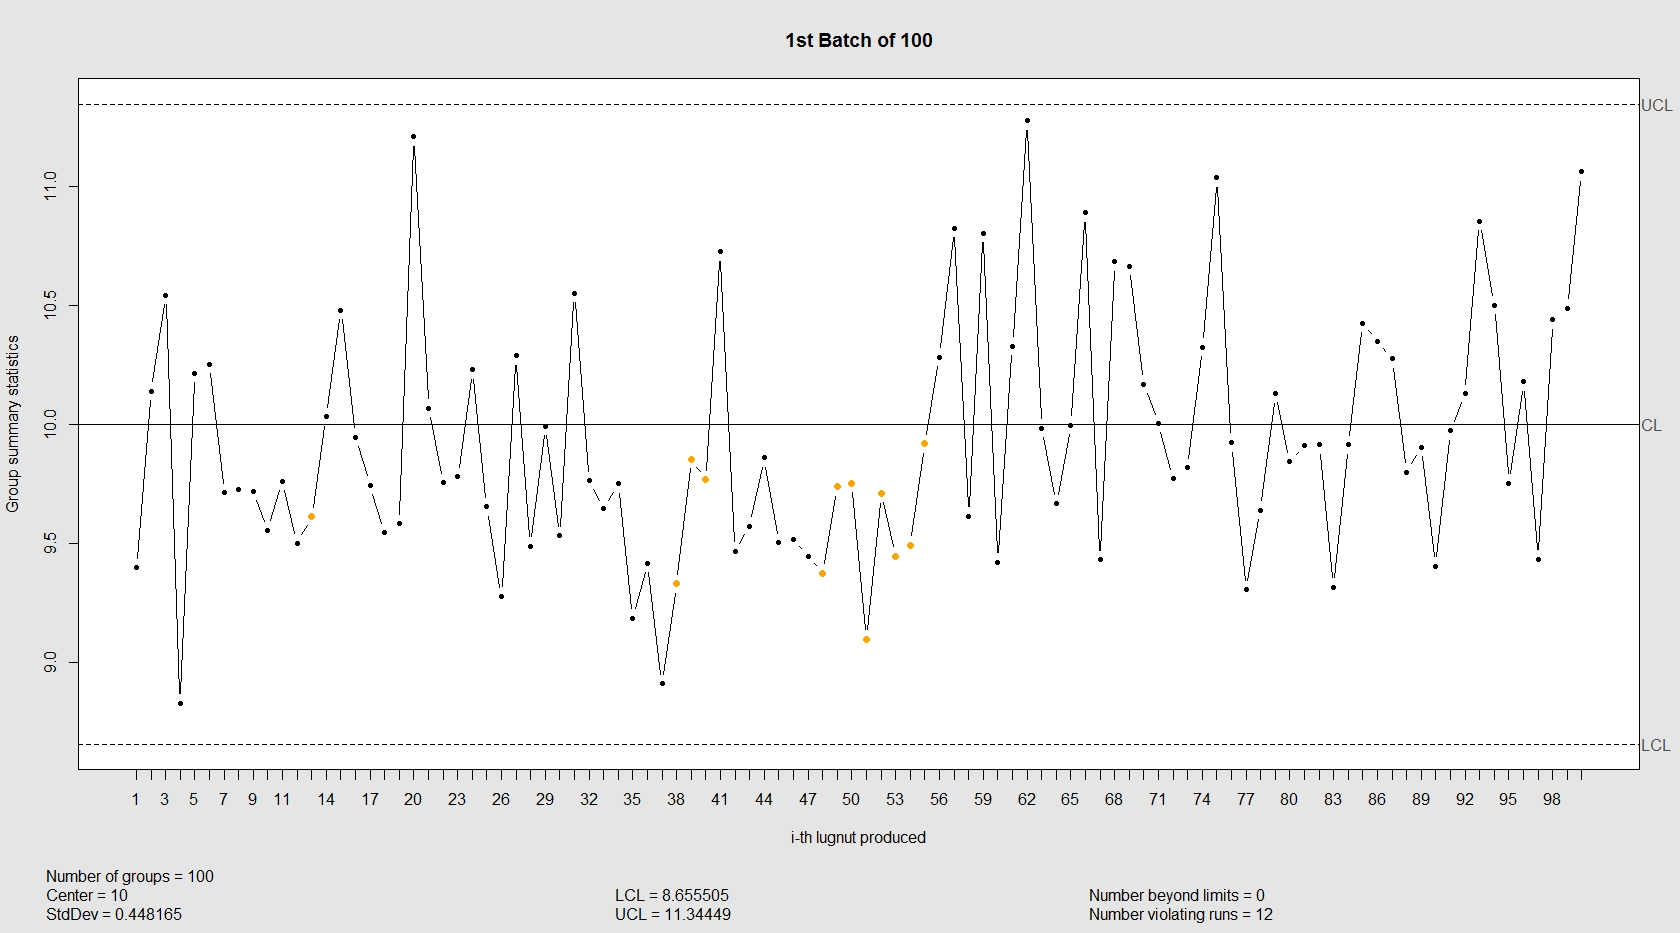
\includegraphics[width=0.8\linewidth]{images/lugnuts1}
	\caption{}
	\label{fig:lugnuts1}
\end{figure}
\begin{figure}[h!]
	\centering
	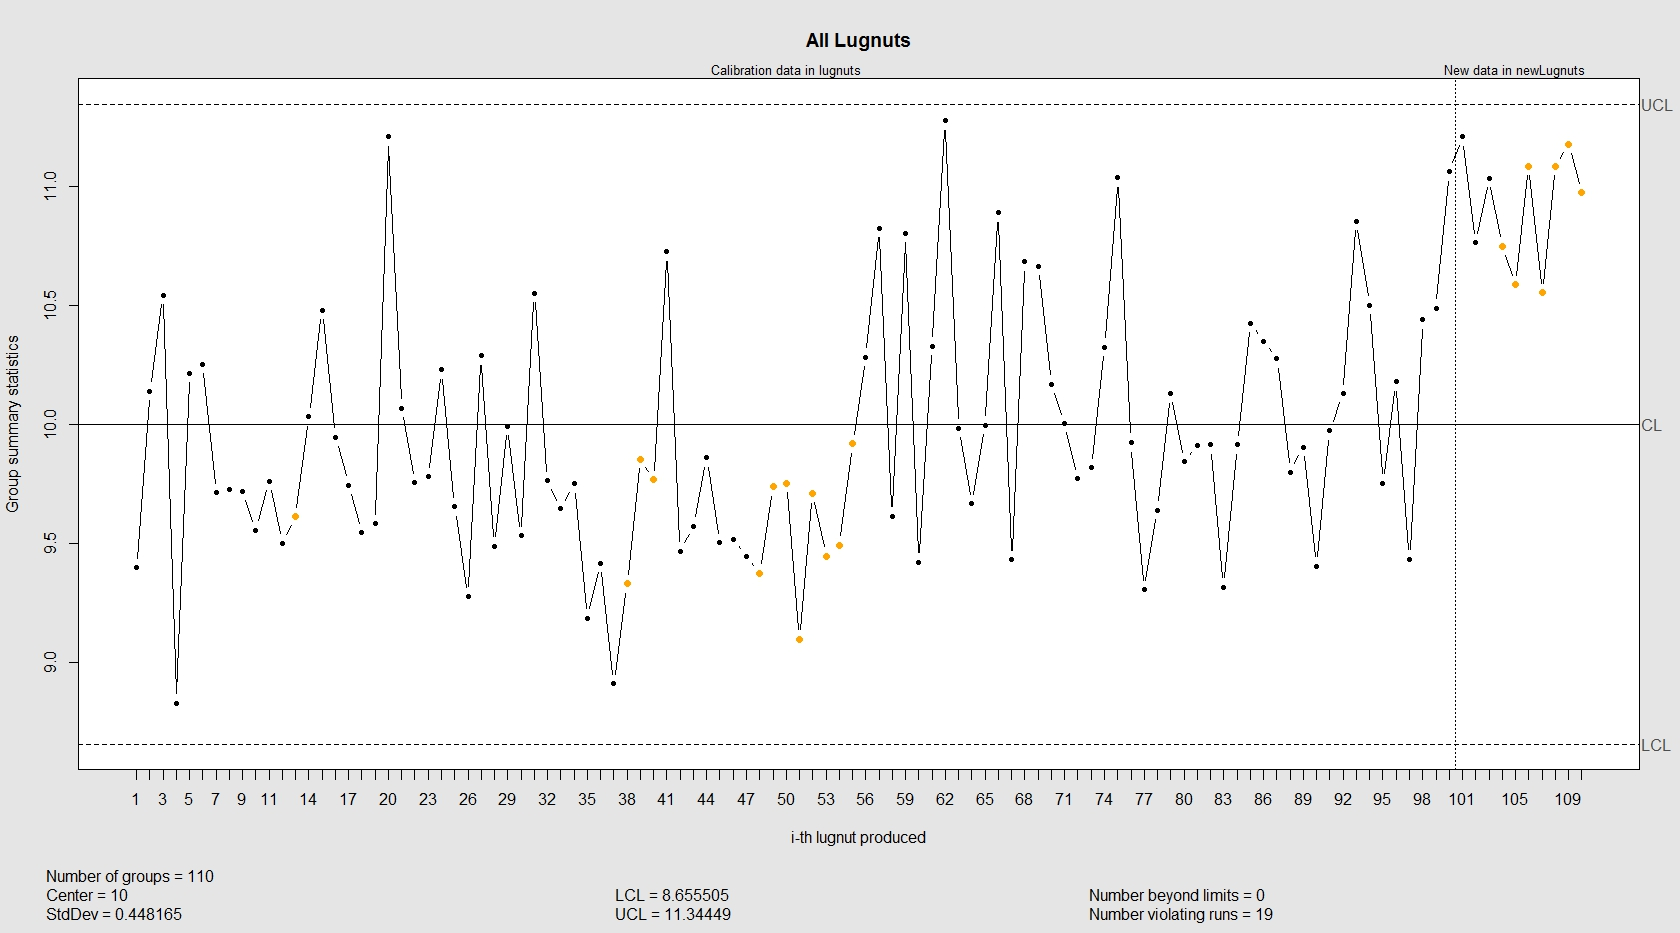
\includegraphics[width=0.8\linewidth]{images/lugnuts2}
	\caption{}
	\label{fig:lugnuts2}
\end{figure}
\newpage
\subsection{Using the \texttt{summary} command}
\begin{framed}
	\begin{verbatim}
	Call:
	qcc(data = lugnuts, type = "xbar.one", center = 10, add.stats = TRUE,     
	title = "1st Batch of 100", xlab = "i-th lugnut produced")
	
	xbar.one chart for lugnuts 
	
	Summary of group statistics:
	Min. 1st Qu.  Median    Mean 3rd Qu.    Max. 
	8.827   9.552   9.808   9.922  10.240  11.270 
	
	Group sample size:  1
	Number of groups:  100
	Center of group statistics:  10
	Standard deviation:  0.448165 
	
	Control limits:
	LCL      UCL
	8.655505 11.34449
	\end{verbatim}
\end{framed}
\begin{framed}
	\begin{verbatim}
	Call:
	qcc(data = lugnuts, type = "xbar.one", center = 10, newdata = newLugnuts,     
	add.stats = TRUE, title = "All Lugnuts", xlab = "i-th lugnut produced")
	
	xbar.one chart for lugnuts 
	.....
	
	Summary of group statistics in newLugnuts:
	Min. 1st Qu.  Median    Mean 3rd Qu.    Max. 
	10.55   10.75   11.00   10.92   11.08   11.21 
	
	Group sample size:  1
	Number of groups:  10 
	
	Control limits:
	LCL      UCL
	8.655505 11.34449
	
	\end{verbatim}
\end{framed}
\newpage

\subsubsection{Example used by Drew Conway}
\begin{figure}[h!]
	\centering
	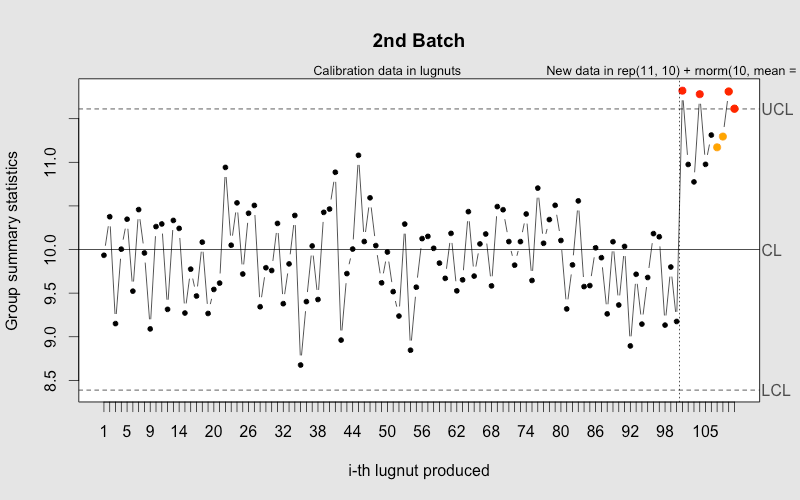
\includegraphics[width=0.7\linewidth]{./qcc_holdout2}
	\caption{}
	\label{fig:qcc_holdout2}
\end{figure}
\begin{framed}
	\begin{verbatim} 
	
	lugnuts <- rep(10, 100) + rnorm(100, mean=0, sd=0.5)
	qcc(lugnuts, newdata=rep(11, 10) + rnorm(10, mean=0, sd=0.5),
	type="xbar.one", center=10, 
	add.stats=FALSE, title="2nd Batch", 
	xlab="i-th lugnut produced")
	\end{verbatim}
\end{framed}

\subsubsection{Remarks}
{\large
	\begin{itemize}
		\item \texttt{newdata}
		\item \texttt{add.stats }
	\end{itemize}}
	
	
	
	
	
	\subsection{Using \texttt{R}}
	{
		\large
		Advantages of using R statistical program along with the \textbf{qcc} package:
		\begin{itemize}
			\item There are several packages for interfacing with databases, RODBC being a common and useful one on MS windows.
			\item Allows of automation: you can program a regular event loop to check for new data and run a new set of charts and notifications if there is new data.
			\item The \textbf{mail} and \textbf{sendmailR} packages were designed to automatically send e-mails with regular reports and warning messages.
			\item It produces the standard SPC charts, these can go to the screen or a file to be sent out.
			\item Bespokes tests can be program for out of control signals
			\item Full programming language with common (and uncommon) statistics so you can pre-proccess you data in many ways to reduce dimension.
			\item You can have multiple instances running on multiple or a single computer, each processing for a single department, or you can combine it all into one script to run for all the departments.
		\end{itemize}
	}
	%------------------------------------------------------ % 
	
	
	
	
	
	

\chapter{Multivariate SPC}
\section{Multivariate Control Charts}
{\large
%MSQC book Part 2
\begin{itemize}
\item With the enhancements in data acquisition systems it is usual to deal with processes
with more than one correlated quality characteristic to be monitored. 
\item A common
practice is to control the stability of the process using univariate control charts. 
\item This
practice increases the probability of false alarm of special cause of variation.
\item Therefore, the analysis should be performed through a multivariate approach;
that is, the variables must be analyzed together, not independently.
\end{itemize}

\subsection{Multivariate Control Charts}
% http://www.jmp.com/support/help/Multivariate_Control_Charts.shtml
{\large\begin{itemize}
\item Multivariate control charts monitor multiple process characteristics. Independent variables can be charted individually, but if the variables are correlated, a multivariate chart is needed to determine whether the process is in control. 
\item Multivariate control charts can detect shifts in the mean or the relationship between several related variables.
\item 
The multivariate control chart plots Hotelling’s T2 statistic. The calculation for the control limit differs based on whether targets have been specified.
\end{itemize}}

\subsection{The MSQC package}

In his book, Edgar Santos-Fernandez present the multivariate normal distribution, the data structure
of the multivariate problems dealt in this book, the mult.chart function that allows
the computation in R, and the most used multivariate control charts:
}
\begin{itemize}
\item The control ellipsoid or w2 control chart
\item The T2 or Hotelling chart
\item The Multivariate Exponentially Weighted Moving Average (MEWMA) chart
\item The Multivariate Cumulative Sum (MCUSUM) chart
\item The chart based on Principal Components Analysis (PCA)
\end{itemize} 

\subsection{The \texttt{mult.chart} Function}
The performing of the multivariate control chart in R can be carried out with the
function mult.chart which is a general function that allows to compute the most
accepted and diversified continuous multivariate chart such as

\begin{itemize} 
\item $\chi^2$
\item Hotelling $T^2$
\item MEWMA
\item MCUSUM according to Crosier (1988)
\item MCUSUM by Pignatiello and Runger (1990)
\end{itemize}
Finally the function \texttt{mult.chart} returns:

\begin{itemize} 
\item The T2 statistics
\item The Upper Control Limit (UCL)
\item The sample covariance matrix (S)
\item The mean vector (Xmv)
\item And if any point falls outside of the UCL and its decomposition
\end{itemize}

\begin{framed}
\begin{verbatim}
mult.chart(dowel1, type = "chi", alpha = 0.05)
\end{verbatim}
\end{framed}

\subsection{T2 control chart}
\large
The origin of the T2 control chart dates back to the pioneer works of Harold Hotelling
who applied this method to the bombsight problem in Second World War. The
Hotelling (1947) procedure has become without doubt the most applied in multivariate
process control and it is the multivariate analogous of the Shewhart control chart.
For that reason, it is also known as multivariate Shewhart control chart.
\begin{framed}
\begin{verbatim}
data("carbon1")
mult.chart(type = "t2", carbon1)
mult.chart(type = "t2", carbon1)$t2
\end{verbatim}
\end{framed}
\newpage

%--------------------------------------------------------------- %
\newpage
\subsection{\texttt{mqcc} Example}
\begin{framed}
\begin{verbatim}
# library(mqcc)
# Ryan (2000, Table 9.2) data with p = 2 variables, 
#  m = 20 samples, n = 4 sample size:

X1 = matrix(c(72, 56, 55, 44, 97, 83, 47, 88, 57, 26, 46,
49, 71, 71, 67, 55, 49, 72, 61, 35, 84, 87, 73, 80, 26, 89, 66,
50, 47, 39, 27, 62, 63, 58, 69, 63, 51, 80, 74, 38, 79, 33, 22,
54, 48, 91, 53, 84, 41, 52, 63, 78, 82, 69, 70, 72, 55, 61, 62,
41, 49, 42, 60, 74, 58, 62, 58, 69, 46, 48, 34, 87, 55, 70, 94,
49, 76, 59, 57, 46), ncol = 4)

X2 = matrix(c(23, 14, 13, 9, 36, 30, 12, 31, 14, 7, 10,
11, 22, 21, 18, 15, 13, 22, 19, 10, 30, 31, 22, 28, 10, 35, 18,
11, 10, 11, 8, 20, 16, 19, 19, 16, 14, 28, 20, 11, 28, 8, 6,
15, 14, 36, 14, 30, 8, 35, 19, 27, 31, 17, 18, 20, 16, 18, 16,
13, 10, 9, 16, 25, 15, 18, 16, 19, 10, 30, 9, 31, 15, 20, 35,
12, 26, 17, 14, 16), ncol = 4)

X = list(X1 = X1, X2 = X2)
q = mqcc(X, type = "T2")
summary(q)
\end{verbatim}
\end{framed}
\begin{figure}[h!]
\centering
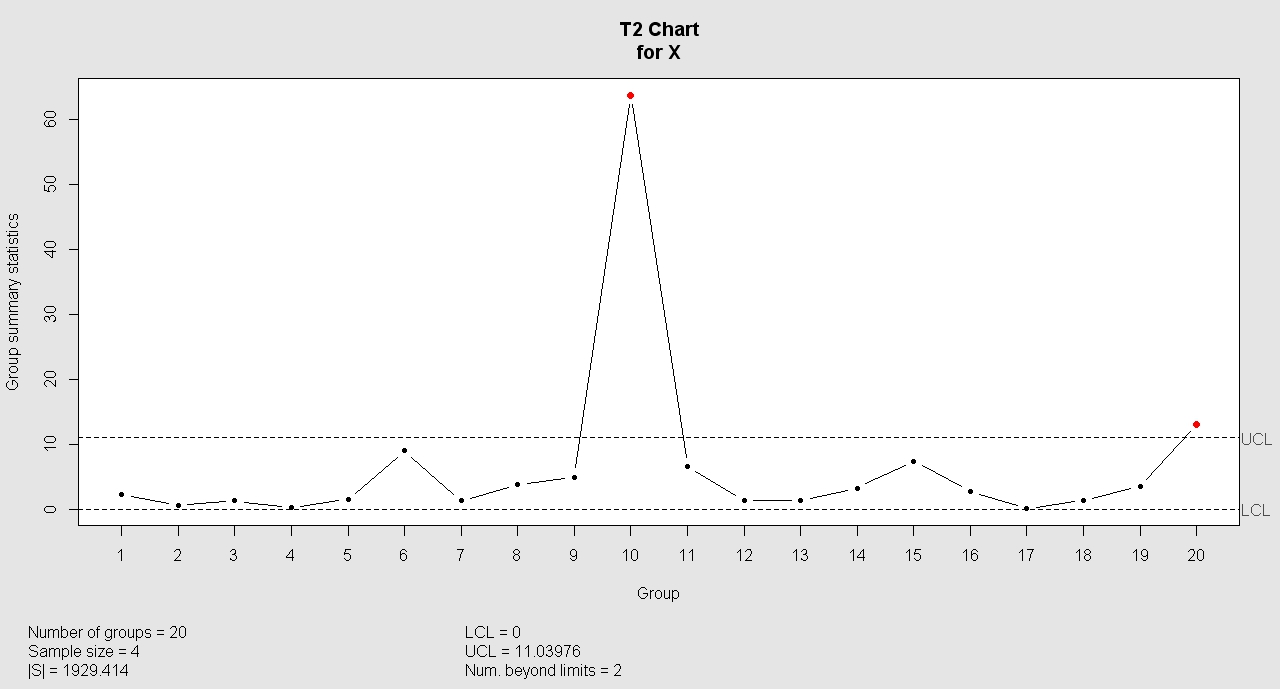
\includegraphics[width=0.9\linewidth]{images/mqccplot1}
\caption{}
\label{fig:mqccplot1}
\end{figure}
\newpage
\begin{verbatim}
Call:
mqcc(data = X, type = "T2")

T2 chart for X 

Summary of group statistics:
   Min. 1st Qu.  Median    Mean 3rd Qu.    Max. 
 0.1243  1.3250  2.5030  6.4700  5.3490 63.7600 

Number of variables:  2
Number of groups:  20
Group sample size:  4

Center: 
     X1      X2 
60.3750 18.4875 

Covariance matrix:
         X1        X2
X1 222.0333 103.11667
X2 103.1167  56.57917
|S|:  1929.414 

Control limits:
 LCL      UCL
   0 11.03976

\end{verbatim}

%\subsection{Confidence Region}
%a confidence region is a multi-dimensional generalization of a confidence interval. It is a set of points in an n-dimensional space, often represented as an ellipsoid around a point which is an estimated solution to a problem, although other shapes can occur.
%
%The confidence region is calculated in such a way that if a set of measurements were repeated many times and a confidence region calculated in the same way on each set of measurements, then a certain percentage of the time, on average, (e.g. 95%) the confidence region would include the point representing the "true" values of the set of variables being estimated. However, unless certain assumptions about prior probabilities are made, it does not mean, when one confidence region has been calculated, that there is a 95% probability that the "true" values lie inside the region, since we do not assume any particular probability distribution of the "true" values and we may or may not have other information about where they are likely to lie.
\newpage

\section{The \textbf{qcc} R package - The 7QC tools revisited}

\begin{itemize}
\item The \textbf{qcc} package  was built by Luca Scrucca for nothing but statistical quality control. 
\item It's extremely easy to use. You provide it with data and it tells you which points are considered to be outliers based on the Shewart Rules. 
\item It even color codes them based on how irregular each point is. 
%In the example below you can see that for the last 10 points of the 2nd dataset I shifted he mean of the data from 10 to 11.
% %
\item 
Even though statistical quality control an old topic, statistical quality control is still highly relevant. There are probably have lots of jobs, processes, logs, or databse metric tha could be monitored using control charts.
\end{itemize}


%Yhat Blog


\subsection{qcc : Quality Control Charts}
\textbf{Some Remarks}
\begin{itemize}
\item Shewhart quality control charts for continuous, attribute and count data.
\item Cusum and EWMA charts. 
\item Operating characteristic curves.
\item Process capability analysis. 
\item Pareto chart and cause-and-effect chart. 
\item Multivariate control charts.
\end{itemize}

\subsection{Types of Control Chart supported by qcc}
{
\large
\begin{description}
\item["xbar"]	 	mean -  means of a continuous process variable
\item["R"]	 	range	 ranges of a continuous process variable
\item["S"]	 	standard deviation	 standard deviations of a continuous variable
\item["xbar.one"]	 	mean	 one-at-time data of a continuous process variable
\item["p"]	 	proportion	 proportion of nonconforming units
\item["np"]	 	count	 number of nonconforming units
\item["c"]	 	count	 nonconformities per unit
\item["u"]	 	count	 average nonconformities per unit
\item["g"]	 	count	 number of non-events between events
\end{description}

}

\subsection{Pareto Chart Analysis.}
{
\large 
\begin{itemize}
\item A Pareto chart is a barplot where the categories are ordered in non increasing order, and a line is also added to show the cumulative sum.
\item Quality problems are rarely spread evenly across the different aspects of the production process or different plants. Rather, a few "bad apples" often account for the majority of problems. 
\item This principle has come to be known as the Pareto principle, which basically states that quality losses are mal-distributed in such a way that a small percentage of possible causes are responsible for the majority of the quality problems. 
\item For example, a relatively small number of "dirty" cars are probably responsible for the majority of air pollution; the majority of losses in most companies result from the failure of only one or two products. To illustrate the "bad apples", one plots the Pareto chart,
\end{itemize}
}
\subsection{Pareto Analysis (Implementation with qcc package)}
\begin{framed}
\begin{verbatim}
defect <- c(80, 27, 66, 94, 33)

names(defect) <- c("price code", "schedule date", 
 "supplier code", "contact num.", "part num.")

# 1
pareto.chart(defect, ylab = "Error frequency")

#2
pareto.chart(defect, ylab = "Error frequency", xlab = "Error causes", las=1)

#3
pareto.chart(defect, ylab = "Error frequency", col=rainbow(length(defect)))

#4
pareto.chart(defect, cumperc = seq(0, 100, by = 5), 
    ylab2 = "A finer tickmarks grid")

\end{verbatim}
\end{framed}
\newpage
\textbf{Output to accompany graphs}
\begin{verbatim}
Pareto chart analysis for defect
                Frequency Cum.Freq. Percentage Cum.Percent.
  contact num.         94        94   31.33333     31.33333
  price code           80       174   26.66667     58.00000
  supplier code        66       240   22.00000     80.00000
  part num.            33       273   11.00000     91.00000
  schedule date        27       300    9.00000    100.00000
\end{verbatim}
%------------------------------------------- %
\newpage

\begin{figure}[h!]
\centering
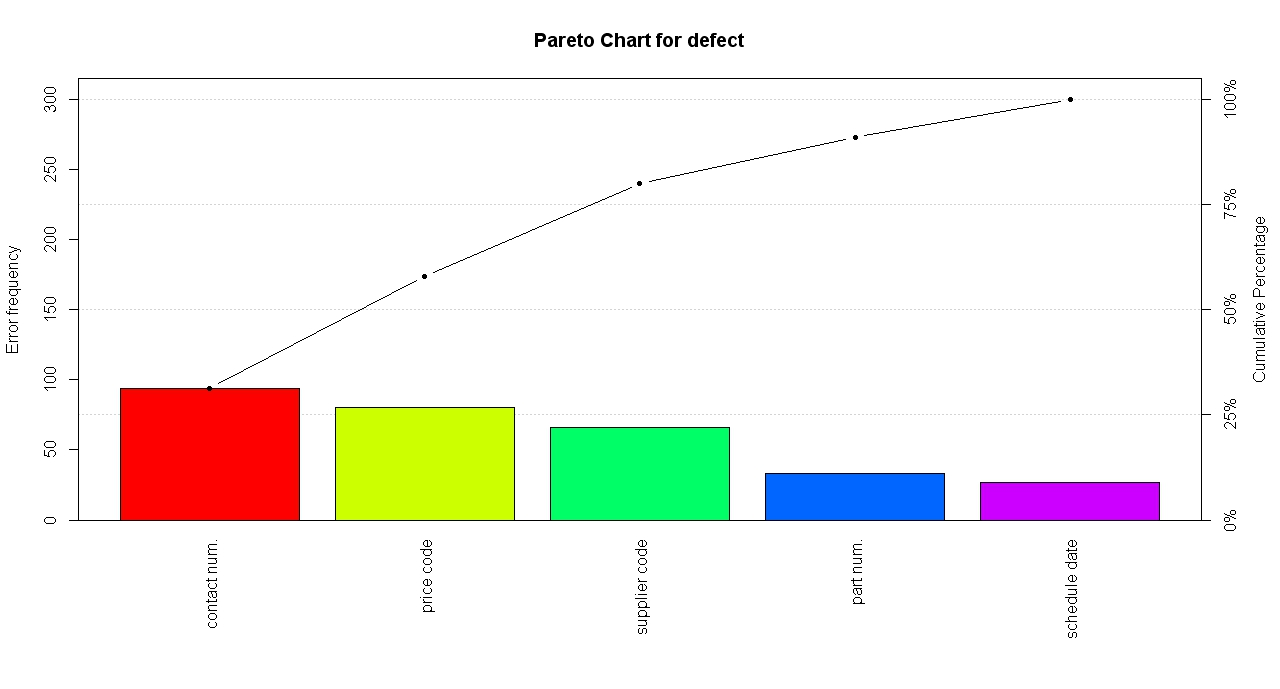
\includegraphics[width=0.8\linewidth]{images/Pareto3}
\caption{Third Implementation}
\label{fig:Pareto3}
\end{figure}

\begin{figure}[h!]
\centering
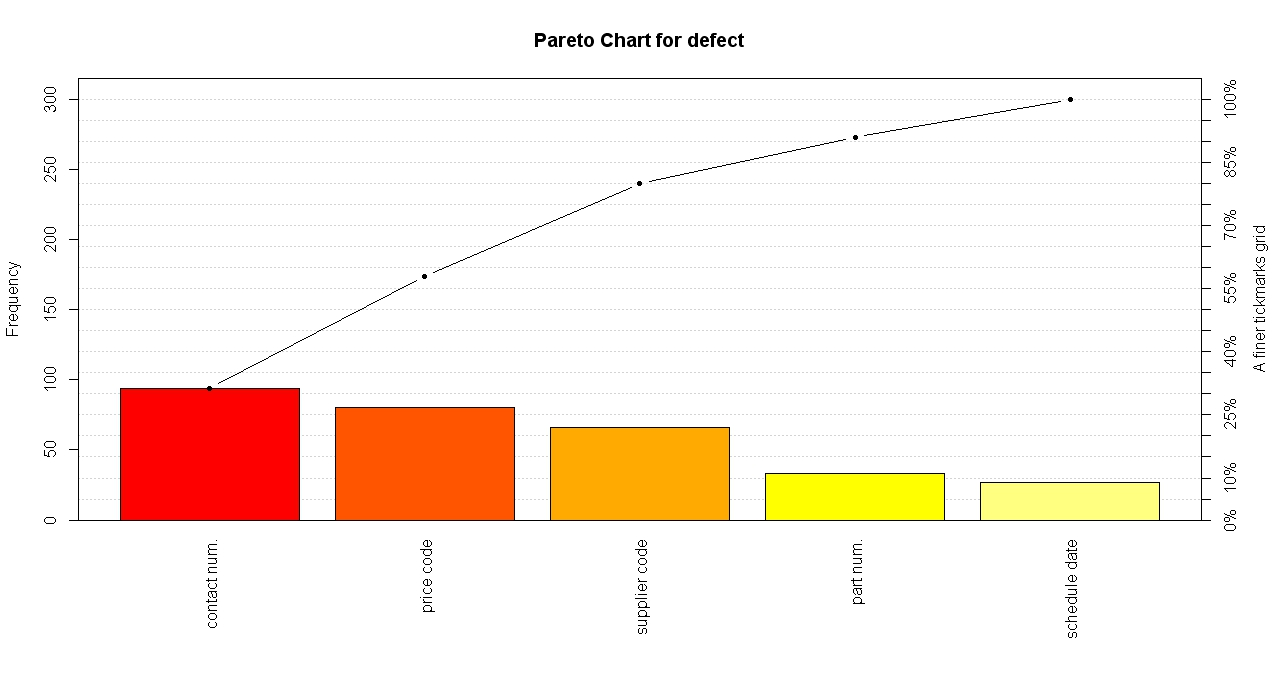
\includegraphics[width=0.8\linewidth]{images/Pareto5}
\caption{Fourth Implementation}
\label{fig:Pareto5}
\end{figure}


\subsection{Cause and Effect Diagrams}
The cause and effect diagram is also known as ``Ishikawa diagram", and has been widely used in
Quality Management. It is one of the Seven Basic Tools of Quality.
\begin{framed}
\begin{verbatim}
cause.and.effect(cause=list(
  Measurements=c("Micrometers", "Microscopes", "Inspectors"),
  Materials=c("Alloys", "Lubricants", "Suppliers"),
  Personnel=c("Shofts", "Supervisors", "Training", "Operators"),
  Environment=c("Condensation", "Moisture"),
  Methods=c("Brake", "Engager", "Angle"),
  Machines=c("Speed", "Lathes", "Bits", "Sockets")),
effect="Surface Flaws")
\end{verbatim}
\end{framed}
\begin{figure}[h!]
\centering
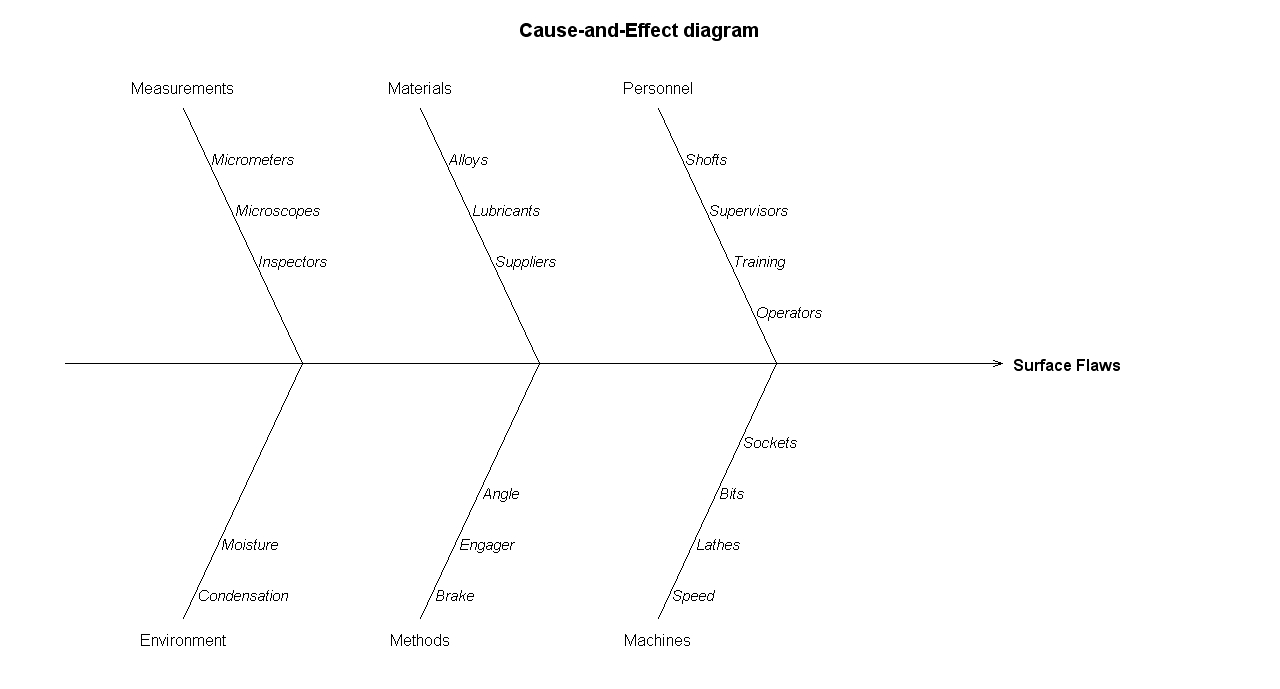
\includegraphics[width=0.7\linewidth]{./qccfishbone}
\caption{}
\label{fig:qccfishbone}
\end{figure}
\newpage
\subsubsection{Implementation with Six Sigma Package}
\begin{framed}
\begin{verbatim}
effect <- "Flight Time"
causes.gr <- c("Operator", "Environment", "Tools", "Design",
"Raw.Material", "Measure.Tool")
causes <- vector(mode = "list", length = length(causes.gr))
causes[1] <- list(c("operator #1", "operator #2", "operator #3"))
causes[2] <- list(c("height", "cleaning"))
causes[3] <- list(c("scissors", "tape"))
causes[4] <- list(c("rotor.length", "rotor.width2", "paperclip"))
causes[5] <- list(c("thickness", "marks"))
causes[6] <- list(c("calibrate", "model"))
ss.ceDiag(effect, causes.gr, causes, sub = "Paper Helicopter Project")
\end{verbatim}
\end{framed}
\begin{figure}[h!]
\centering
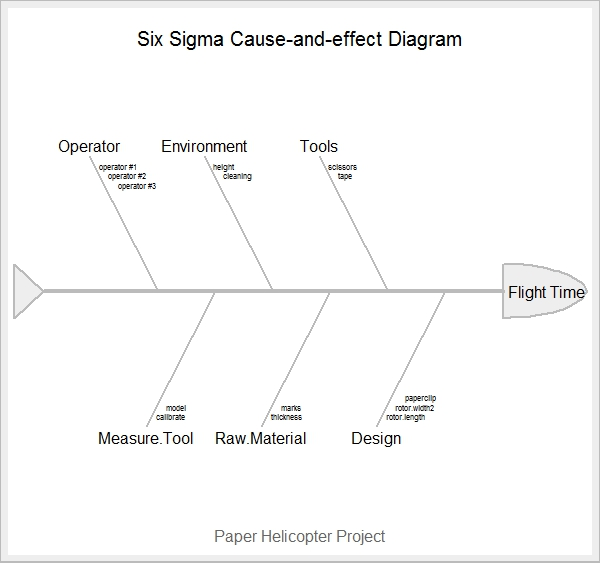
\includegraphics[width=0.7\linewidth]{./Rplot03}
\caption{}
\label{fig:Rplot03}
\end{figure}

\subsection{Constructing Process Maps}
\begin{framed}
\begin{verbatim}
inputs.overall<-c("operators", "tools", "raw material", "facilities")
outputs.overall<-c("helicopter")
steps<-c("INSPECTION", "ASSEMBLY", "TEST", "LABELING")
\end{verbatim}
\end{framed}

\begin{framed}
\begin{verbatim}
#Inputs of process "i" are inputs of process "i+1"
input.output<-vector(mode="list",length=length(steps))
input.output[1]<-list(c("sheets", "..."))
input.output[2]<-list(c("sheets"))
input.output[3]<-list(c("helicopter"))
input.output[4]<-list(c("helicopter"))
\end{verbatim}
\end{framed}
Parameters of each process
\begin{framed}
\begin{verbatim}

x.parameters<-vector(mode="list",length=length(steps))

x.parameters[1]<-list(c(list(c("width", "NC")),list(c("operator", "C")),
                        list(c("Measure pattern", "P")), list(c("discard", "P"))))
x.parameters[2]<-list(c(list(c("operator", "C")),list(c("cut", "P")),
                        list(c("fix", "P")), list(c("rotor.width", "C")),
                        list(c("rotor.length",                                                                                "C")), 
                                                             list(c("paperclip", "C")), list(c("tape", "C"))))
x.parameters[3]<-list(c(list(c("operator", "C")),
list(c("throw", "P")),
                        list(c("discard", "P")), 
                        list(c("environment", "N"))))
x.parameters[4]<-list(c(list(c("operator", "C")),
list(c("label", "P"))))
x.parameters

\end{verbatim}
\end{framed}

\begin{framed}
\begin{verbatim}
#Features of each process
y.features<-vector(mode="list",length=length(steps))
y.features[1]<-list(c(list(c("ok", "Cr"))))
y.features[2]<-list(c(list(c("weight", "Cr"))))
y.features[3]<-list(c(list(c("time", "Cr"))))
y.features[4]<-list(c(list(c("label", "Cr"))))
y.features
ss.pMap(steps, inputs.overall, outputs.overall,
        input.output, x.parameters, y.features,
        sub="Paper Helicopter Project")
\end{verbatim}
\end{framed}
\begin{figure}[h!]
\centering
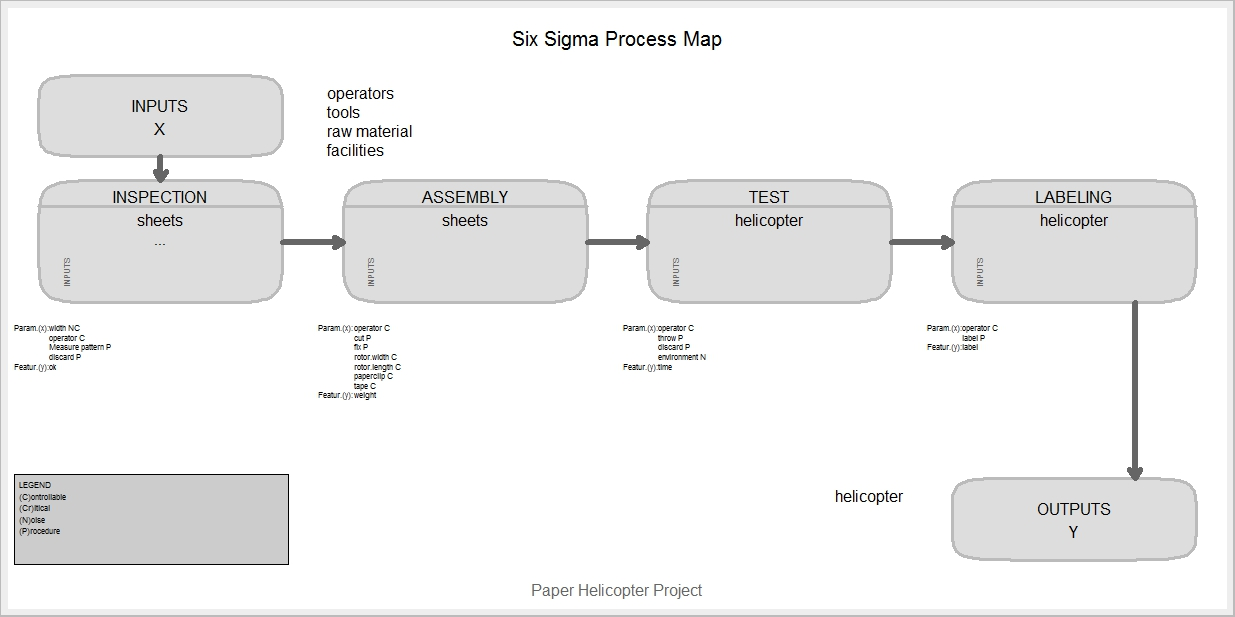
\includegraphics[width=0.9\linewidth]{./SixSigmaProcessMap}
\caption{}
\label{fig:SixSigmaProcessMap}
\end{figure}

\newpage

\section{The \textbf{qcc} R package - Other Types of Graph}




\subsection{Operating Characteristic (OC) Curves}
\begin{itemize}
\item 
The OC Curve is used in sampling inspection. It plots the probability of accepting a batch of items against the quality level of the batch.

\item The figure below shows an 'OC' (Operating Characteristic) Curve for a sample of 50 items taken from a batch of 2000 and using a critical acceptance number 'c' of 2 (the batch will be accepted if there are two or less defectives in the sample).

\item From the curve you can see that there is about a 23\% probability of accepting a batch that contains 8\% of defective items.

\item When designing a sampling plan it is usual to decide on two points, the AQL and LQL and the associated Producer's Risk and Consumer's Risk. The necessary sample size and acceptance number for the curve to pass through these points is then calculated and hence the shape of the curve.

\item OC Curves are mainly associated with sampling inspection but they are also used to find the Average Run Length in control charts.


\item A common supplementary plot to standard quality control charts is the so-called operating characteristic or OC curve (see example below). One question that comes to mind when using standard variable or attribute charts is how sensitive is the current quality control procedure? Put in more specific terms, how likely is it that you will not find a sample (e.g., mean in an X-bar chart) outside the control limits (i.e., accept the production process as "in control"), when, in fact, it has shifted by a certain amount? 

\item This probability is usually referred to as the  (beta) error probability, that is, the probability of erroneously accepting a process (mean, mean proportion, mean rate defectives, etc.) as being "in control." 

\item Note that operating characteristic curves pertain to the false-acceptance probability using the sample-outside-of- control-limits criterion only, and not the runs tests described earlier.


\item Operating characteristic curves are extremely useful for exploring the power of our quality control procedure. The actual decision concerning sample sizes should depend not only on the cost of implementing the plan (e.g., cost per item sampled), but also on the costs resulting from not detecting quality problems. The OC curve allows the engineer to estimate the probabilities of not detecting shifts of certain sizes in the production quality.
\end{itemize}






\newpage
\subsubsection{pistonrings Data}
\begin{framed}
\begin{verbatim}
data(pistonrings); attach(pistonrings);

diameter <- qcc.groups(diameter, sample)
beta <- oc.curves.xbar(qcc(diameter, type="xbar", nsigmas=3, plot=FALSE))
print(round(beta, digits=4))

# or to identify points on the plot use
## Not run: oc.curves.xbar(qcc(diameter, 
    type="xbar", nsigmas=3, plot=FALSE), identify=TRUE)

detach(pistonrings)
\end{verbatim}
\end{framed}

\begin{figure}
\centering
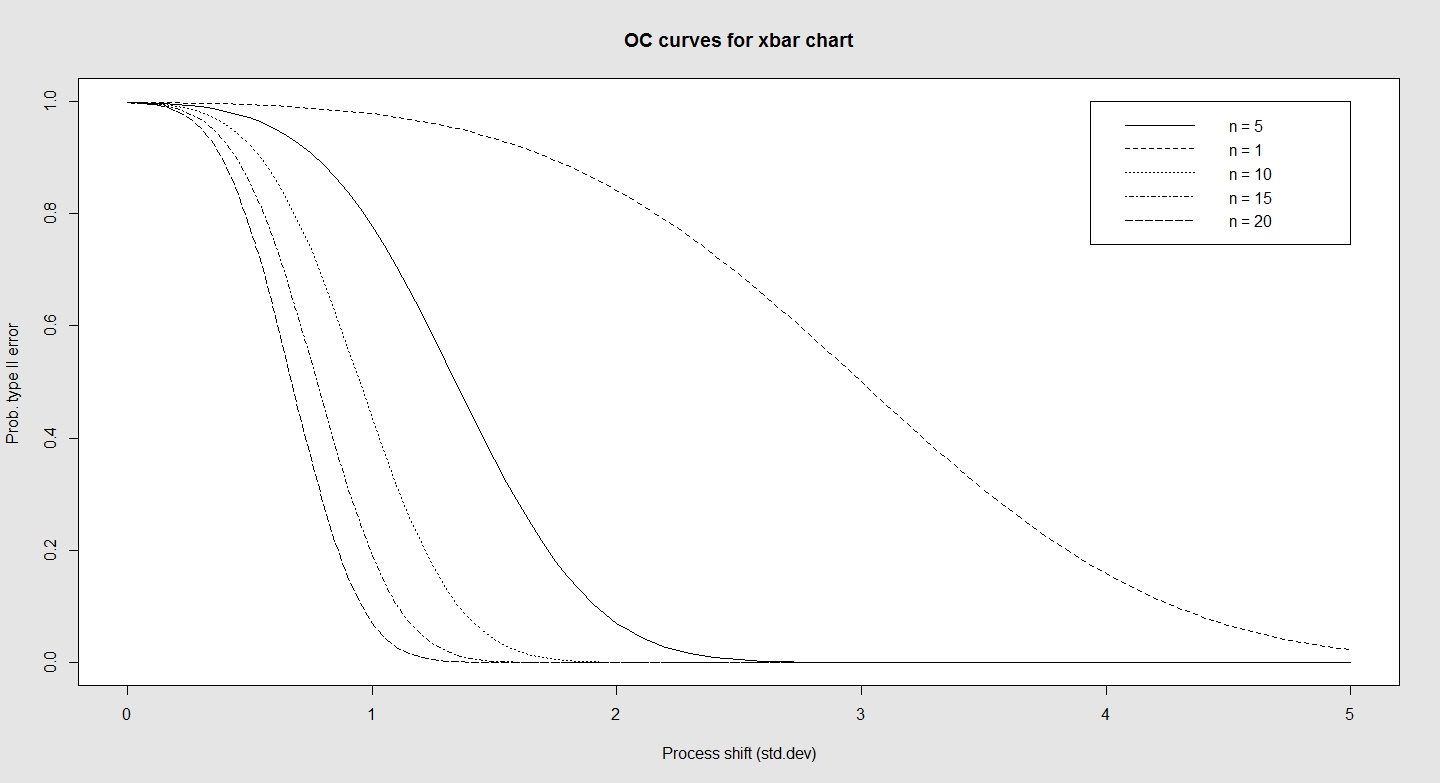
\includegraphics[width=0.7\linewidth]{images/OCpistonrings}
\caption{}
\label{fig:OCpistonrings}
\end{figure}

%\newpage
%\subsubsection{orangejuice Data}
%\begin{framed}
%\begin{verbatim}
%data(orangejuice)
%attach(orangejuice)
%beta <- oc.curves(qcc(D[trial], sizes=size[trial], type="p", plot=FALSE))
%print(round(beta, digits=4))
%# or to identify points on the plot use
%## Not run: oc.curves(qcc(D[trial], sizes=size[trial], type="p", plot=FALSE), identify=TRUE)
%detach(orangejuice)
%\end{verbatim}
%\end{framed}
%\newpage
%\subsubsection{circuit Data}
%\begin{framed}
%\begin{verbatim}
%data(circuit)
%attach(circuit)
%q <- qcc(x[trial], sizes=size[trial], type="c", plot=FALSE)
%beta <- oc.curves(q)
%print(round(beta, digits=4))
%# or to identify points on the plot use
%## Not run: oc.curves(qcc(x[trial], sizes=size[trial], type="c", plot=FALSE), identify=TRUE)
%detach(circuit)
%\end{verbatim}
%\end{framed}
%\newpage
\newpage
\subsection{Moving Average (MA) Chart}

\begin{itemize}
\item To return to the piston ring example, suppose we are mostly interested in detecting small trends across successive sample means. 
\item For example, we may be particularly concerned about machine wear, leading to a slow but constant deterioration of quality (i.e., deviation from specification). 
%The CUSUM chart described above is one way to monitor such trends, and to detect small permanent shifts in the process average. 

\item Another way is to use some weighting scheme that summarizes the means of several successive samples; moving such a weighted mean across the samples will produce a moving average chart (as shown in the following graph).
\end{itemize}
%
%
%
%\subsection{Exponentially-weighted MA (EWMA) Chart}
%The idea of moving averages of successive (adjacent) samples can be generalized. In principle, in order to detect a trend we need to weight successive samples to form a moving average; however, instead of a simple arithmetic moving average, we could compute a geometric moving average (this chart (see graph below) is also called Geometric Moving Average chart, see Montgomery, 1985, 1991).
%-------------------------------------------------- %
\newpage
\subsubsection{GExponentially-weighted MA (EWMA) Chart}
\begin{framed}
\begin{verbatim}

data(pistonrings)
attach(pistonrings)
diameter <- qcc.groups(diameter, sample)
q <- ewma(diameter[1:25,], lambda=0.2, nsigmas=3)
summary(q)

q <- ewma(diameter[1:25,], lambda=0.2, nsigmas=2.7,
newdata=diameter[26:40,], plot = FALSE)
summary(q)

plot(q)
\end{verbatim}
\end{framed}

\begin{figure}[h!]
\centering
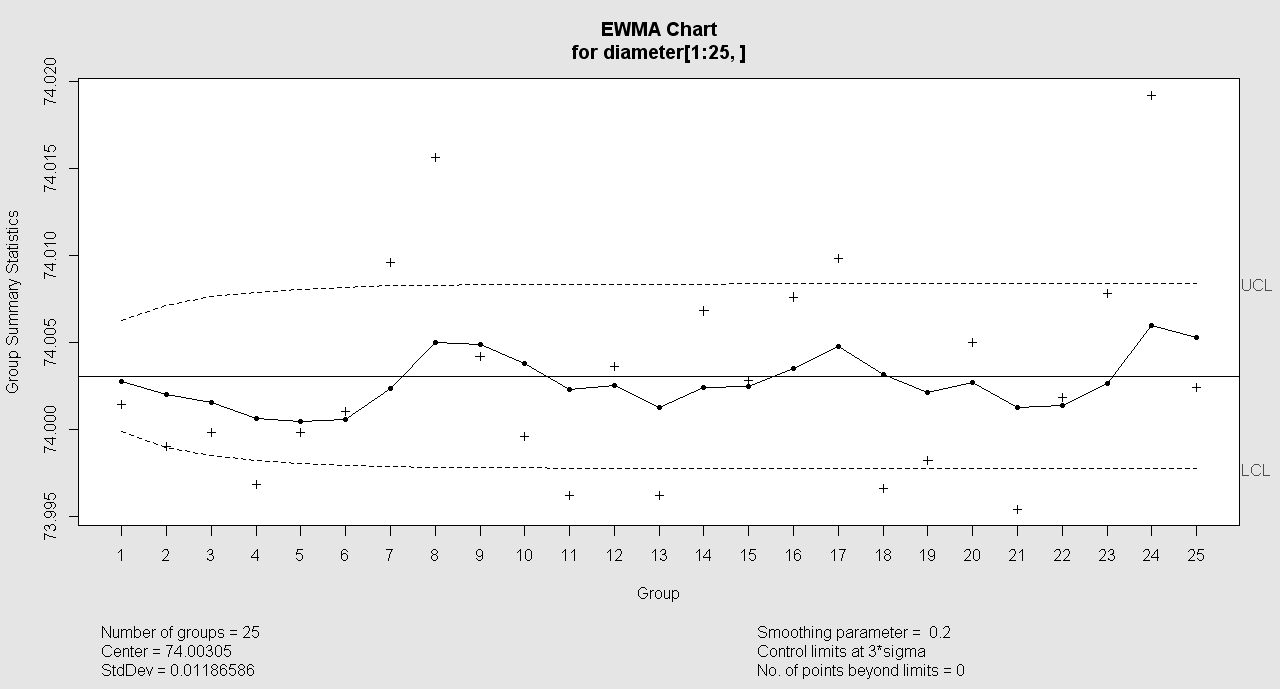
\includegraphics[width=0.6\linewidth]{./qccEWMA1}
\caption{}
\label{fig:qccEWMA1}
\end{figure}
\begin{figure}[h!]
\centering
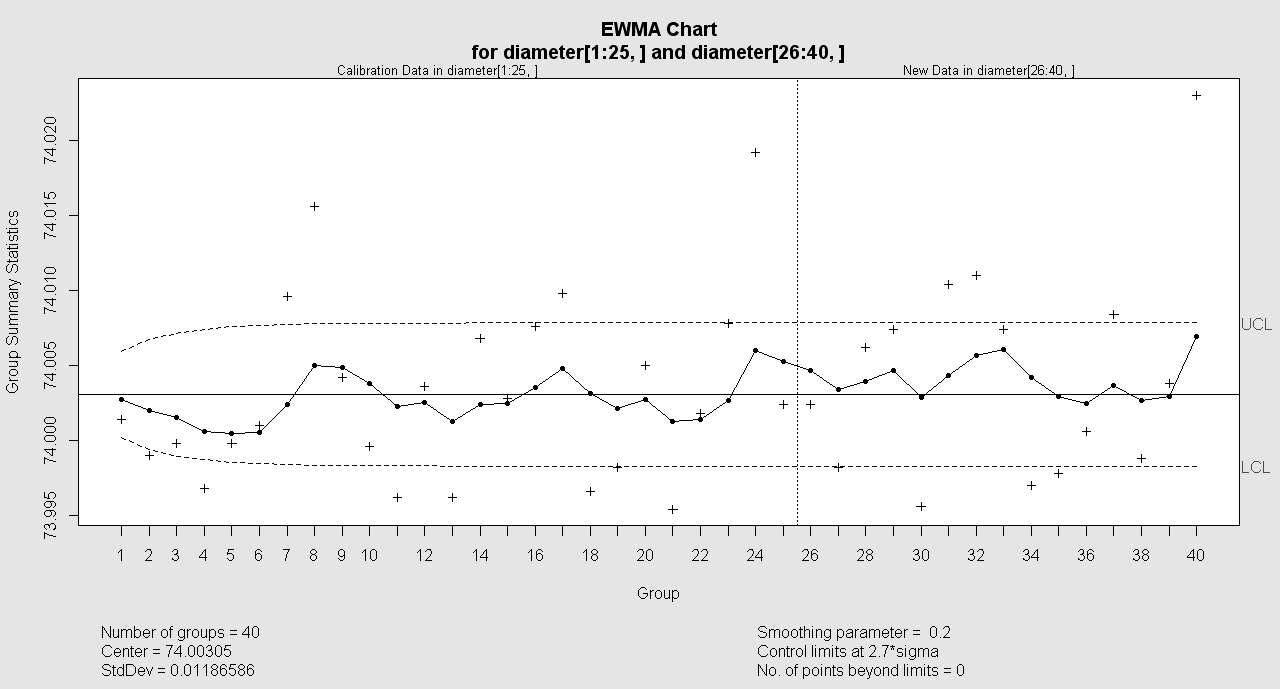
\includegraphics[width=0.6\linewidth]{./qccEWMA2}
\caption{}
\label{fig:qccEWMA2}
\end{figure}
\begin{verbatim}
> summary(q)

Call:
ewma(data = diameter[1:25, ], lambda = 0.2, nsigmas = 2.7, 
newdata = diameter[26:40,     ], plot = FALSE)

ewma chart for diameter[1:25, ] 

Summary of group statistics:
   Min. 1st Qu.  Median    Mean 3rd Qu.    Max. 
  74.00   74.00   74.00   74.00   74.01   74.02 

Group sample size:  5
Number of groups:  25
Center of group statistics:  74.00305
Standard deviation:  0.01186586 

Summary of group statistics in diameter[26:40, ]:
   Min. 1st Qu.  Median    Mean 3rd Qu.    Max. 
  74.00   74.00   74.00   74.00   74.01   74.02 

Group sample size:  5
Number of groups:  15 

Smoothing parameter: 0.2 
Control limits:
         LCL      UCL
1   74.00018 74.00591
2   73.99938 74.00672
...                  
40  73.99827 74.00782

\end{verbatim}
\newpage
\subsubsection{EWMA : Individual observations}
{
\large
\begin{framed}
\begin{verbatim}
x <- c(33.75, 33.05, 34, 33.81, 33.46, 34.02, 33.68, 33.27, 33.49, 33.20,
33.62, 33.00, 33.54, 33.12, 33.84) # viscosity data (Montgomery, pag. 242)
q <- ewma(x, lambda=0.2, nsigmas=2.7)
summary(q)
\end{verbatim}
\end{framed}

\begin{framed}
\begin{verbatim}
x <- 1:50
y <- rnorm(50, sin(x/5), 0.5)
plot(x,y,pch=16,col="blue",font.lab=2)
lines(ewmaSmooth(x,y,lambda=0.1), col="red")
abline(h=mean(y),col="green",lty=2)
title("EWMA Smoother")
\end{verbatim}
\end{framed}
}
\begin{figure}
\centering
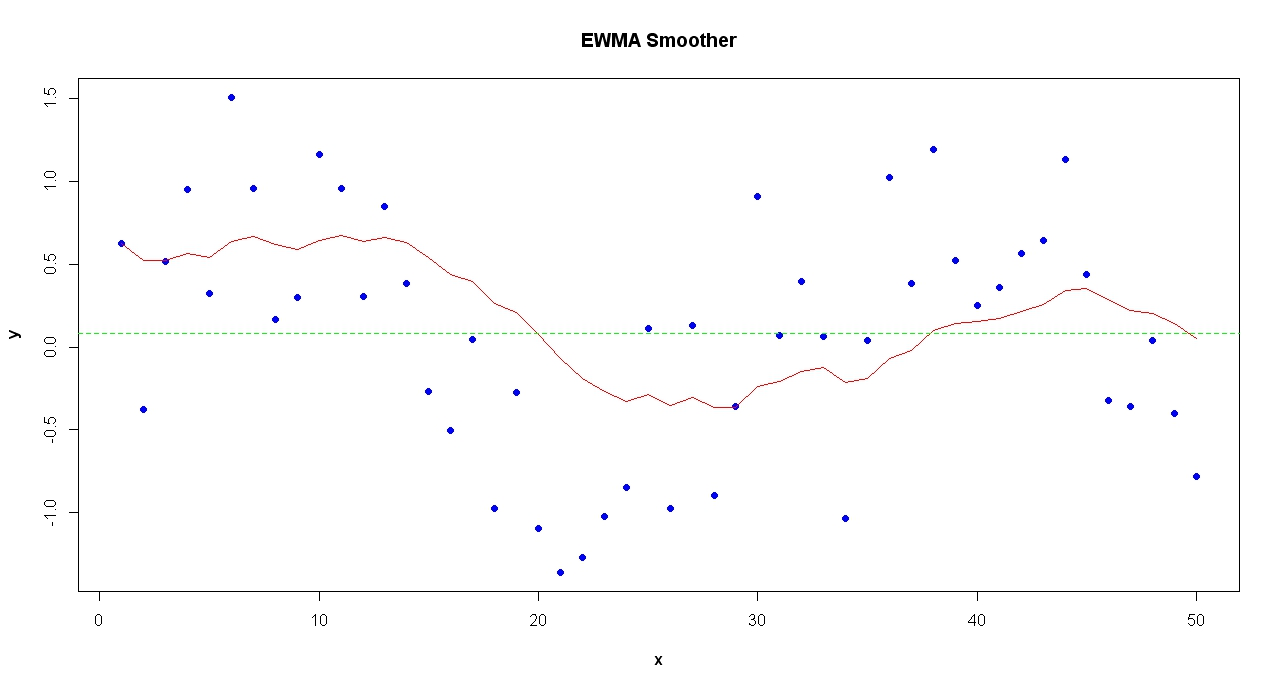
\includegraphics[width=0.7\linewidth]{./qccEWMAsmoother}
\caption{}
\label{fig:qccEWMAsmoother}
\end{figure}
%--------------------------------------------------------------- %
\newpage
\subsection{CUSUM charts}
\begin{itemize}
\item CUSUM charts, while not as intuitive and simple to operate as Shewhart charts, have been shown to be more efficient in detecting small shifts in the mean of a process. \item In particular, analyzing ARL's for CUSUM control charts shows that they are better than Shewhart control charts when it is desired to detect shifts in the mean that are 2 sigma or less.
\end{itemize}



% http://www.itl.nist.gov/div898/handbook/pmc/section3/pmc323.htm
\newpage
\begin{figure}[h!]
\centering
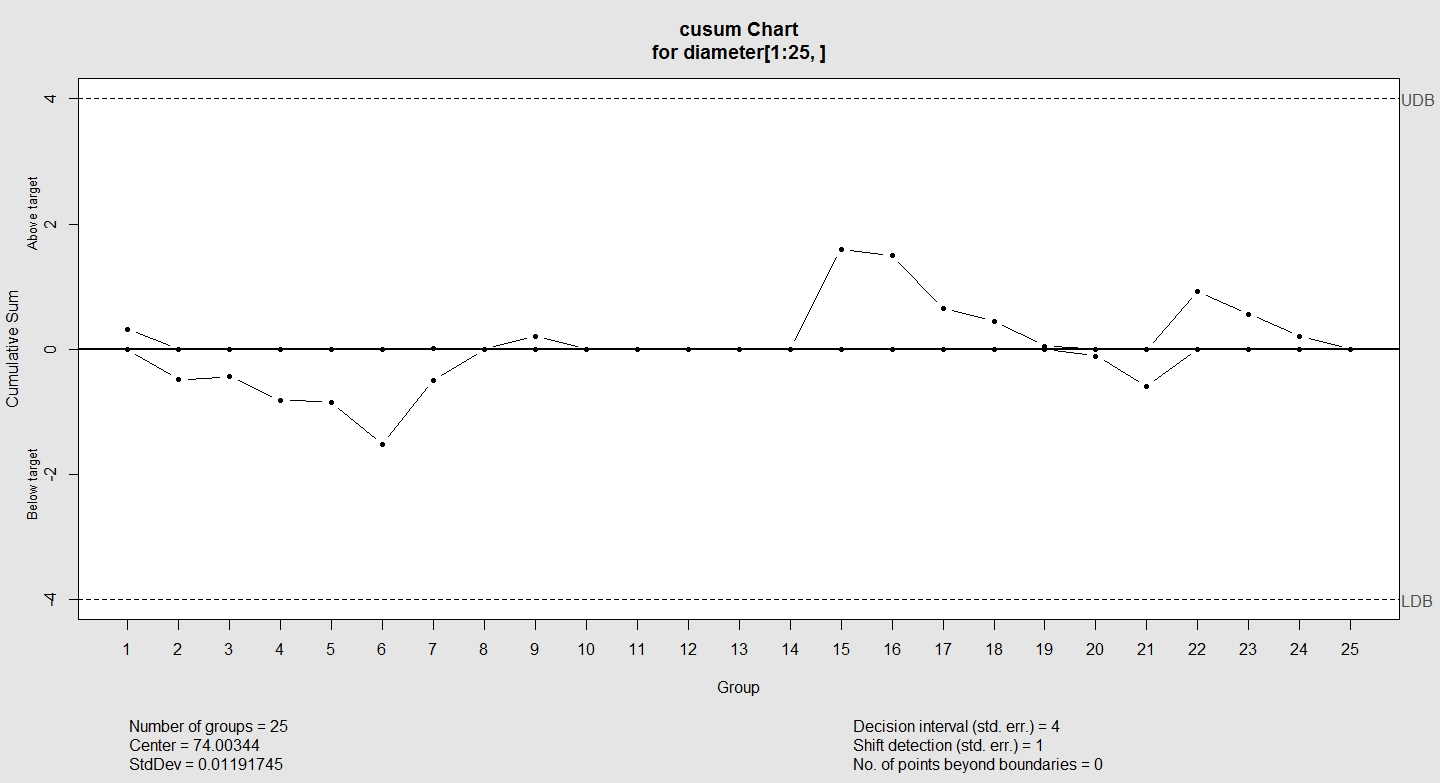
\includegraphics[width=0.7\linewidth]{images/CUSUMorings1}
\caption{}
\label{fig:CUSUMorings1}
\end{figure}

\begin{figure}[h!]
\centering
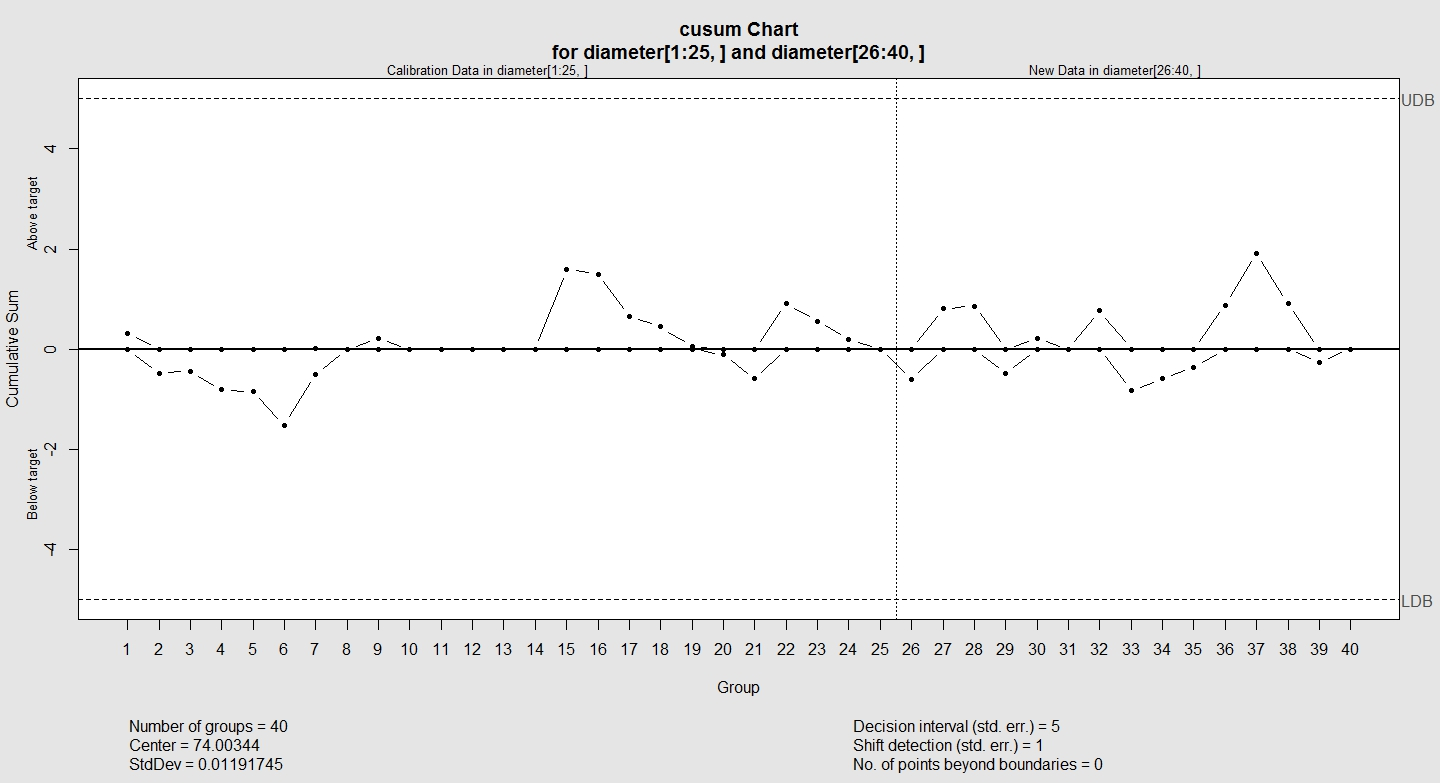
\includegraphics[width=0.7\linewidth]{images/CUSUMorings2}
\caption{}
\label{fig:CUSUMorings2}
\end{figure}


%-------------------------------------------------------------- %
\newpage
\subsection{Individual/Moving-Range chart}
% http://en.wikipedia.org/wiki/Shewhart_individuals_control_chart
\begin{itemize}
\item The individual/moving-range chart is a type of control chart used to monitor variables data from a business or industrial process for which it is impractical to use rational subgroups.

\item The chart is necessary in the following situations:
\begin{itemize}
\item[$\ast$] Where automation allows inspection of each unit, so rational subgrouping has less benefit.
\item[$\ast$]Where production is slow so that waiting for enough samples to make a rational subgroup unacceptably delays monitoring
\item[$\ast$] For processes that produce homogeneous batches (e.g., chemical) where repeat measurements vary primarily because of measurement error
\end{itemize}
\item The "chart" actually consists of a pair of charts: one, the individuals chart, displays the individual measured values; the other, the moving range chart, displays the difference from one point to the next. 
\item As with other control charts, these two charts enable the user to monitor a process for shifts in the process that alter the mean or variance of the measured statistic.
\end{itemize}
\newpage
\chapter{Process Capability}
\section{Process Capability}
Process capability is the measure of process performance. Capability refers to the ability of a process to make parts that are well within engineering specifications. A capability study is done to answer the questions, \textit{``Does the process need to be improved?"} and  \textit{``How much does the process need to be improved?"}

To define the study of process capability from another perspective, a capability study is a technique for analyzing the random variability found in a production process. In every manufacturing process there is variability. This variability may be large or small, but it is always present. It can be divided into two types:

\begin{itemize}
	\item Variability due to common (random) causes
	\item Variability due to assignable (special) causes
\end{itemize}
%----------------------------------------------------------------------------------------------%
The first type of variability can be expected to occur naturally within a process. It is attributed to common causes that behave like a constant system of chances. These chances form a unique and describable distribution. This variability can never be completely eliminated from a process. Variability due to assignable causes, on the other hand, refers to the variation that can be linked to specific or special causes. If these causes, or factors, are modified or controlled properly, the process variability associated with them can be eliminated. Assignable causes cannot be described by a single distribution.
%----------------------------------------------------------------------------------------------%
\subsection{Capability Study} 
A capability study measures the performance potential of a process when no assignable causes are present (when it is in statistical control). Since the inherent variability of the process can be described by a unique distribution, usually a normal distribution, capability can be evaluated by utilizing this distribution’s properties. Simply put, capability is expressed as the proportion of in-specification process output to total process input.

Capability calculations allow predictions to be made regarding quality, enabling manufacturers to take a preventive approach to defects. This statistical approach contrasts to the traditional approach to manufacturing, which is a two-step process: production personnel make the product, and quality control personnel inspect and eliminate those products that do not meet specifications. This is wasteful and expensive, since it allows time and materials to be invested in products that are not always usable. It is also unreliable, since even 100\% inspection would fail to catch all defective products.
%----------------------------------------------------------------------------------------------%
Control Limits are Not an Indication of Capability

Those new to SPC often believe they don’t need capability indices. They think they can compare the control limits to the specification limits instead. This is not true, because control limits look at the distribution of averages and capability indices look at the distribution of individuals. The distribution of individuals will always spread out further than the distribution of averages (see figure below). 
%--------------------------------------------------------------------------------------------------%
\subsection{What is Process Capability?}

Distribution of averages compared to distribution of individuals, for the same sample data. Control limits (based on averages) would probably be inside specification limits, even though many parts are out of specification. This shows why you should not compare control limits to specification limits.

Therefore, the control limits are often within the specification limits, but the $\pm 3$ Sigma distribution of parts is not.  Subgroup averages follow more closely a normal distribution. This is why we can create control charts for processes that are not normally distributed. But averages cannot be used for capability calculations, because capability concerns itself with individual parts, or samples from a process. After all, parts, not averages, get shipped.

\subsection{Capability Indices}

\begin{description}
	\item[Capability] — The uniformity of product which a process is capable of producing. Can be expressed numerically using CP, CR, CpK, and Zmax/3 when the data is normally distributed.
	
	\item[CP] — For process capability studies: CP is a capability index defined by the formula. CP shows the process capability potential but does not consider how centered the process is. CP may range in value from 0 to infinity, with a large value indicating greater potential capability. A value of 1.33 or greater is usually desired.
	
	\item[CR] — For process capability studies: the inverse of CP, CR can range from 0 to infinity in value, with a smaller value indicating a more capable process.
	
	\item[CpK] — For process capability studies: an index combining CP and K to indicate whether the process will produce units within the tolerance limits. CpK has a value equal to CP if the process is centered on the nominal; if CpK is negative, the process mean is outside the specification limits; if CpK is between 0 and 1, then some of the 6 sigma spread falls outside the tolerance limits. If CpK is larger than 1, the 6 sigma spread is completely within the tolerance limits. A value of 1.33 or greater is usually desired.
\end{description}
%---------------------------------------------------------------------------------------------------%
\newpage
\subsection{Interpreting Capability Indices}
\begin{itemize}
	\item The greater the CpK value, the better. A CpK greater than 1.0 means that the $6\sigma  (\pm 3\sigma)$ spread of the data falls completely within the specification limits. A CpK of 1.0 means that one end of the $6\sigma$ spread falls on a specification limit. A CpK between 0 and 1 means that part of the $6\sigma$  spread falls outside the specification limits. A negative CpK indicates that the mean of the data is not between the specification limits.
	
	\item Since a CpK of 1.0 indicates that 99.73\% of the parts produced are within specification limits, in this process it is likely that only about 3 out of 1,000 need to be scrapped or rejected. Why bother to improve the process beyond this point, since it will produce no reduction in scrap or reject costs? Improvement beyond just meeting specification may greatly improve product performance, cut warranty costs, or avoid assembly problems.
	
	\item
	Many companies are demanding CpK indexes of 1.33 or 2.0 of their suppliers’ products. A CpK of 1.33 means that the difference between the mean and specification limit is $4\sigma$  (since 1.33 is 4/3). With a CpK of 1.33, 99.994\% of the product is within specification. Similarly a CpK of 2.0 is $6\sigma$  between the mean and specification limit (since 2.0 is 6/3). 
	\item 
	This improvement from 1.33 to 2.0 or better is sometimes justified to produce more product near the optimal target. Depending on the process or part, this may improve product performance, product life, customer satisfaction, or reduce warranty costs or assembly problems.
	\item
	Continually higher CpK indexes for every part or process is not the goal, since that is almost never economically justifiable. A cost/benefit analysis that includes customer satisfaction and other true costs of quality is recommended to determine which processes should be improved and how much improvement is economically attractive.
\end{itemize}
\newpage
\section{Process Capability}
Process capability is the measure of process performance. Capability refers to the ability of a process to make parts that are well within engineering specifications. A capability study is done to answer the questions, \textit{``Does the process need to be improved?"} and  \textit{``How much does the process need to be improved?"}

To define the study of process capability from another perspective, a capability study is a technique for analyzing the random variability found in a production process. In every manufacturing process there is variability. This variability may be large or small, but it is always present. It can be divided into two types:

\begin{itemize}
\item Variability due to common (random) causes
\item Variability due to assignable (special) causes
\end{itemize}
%----------------------------------------------------------------------------------------------%
The first type of variability can be expected to occur naturally within a process. It is attributed to common causes that behave like a constant system of chances. These chances form a unique and describable distribution. This variability can never be completely eliminated from a process. Variability due to assignable causes, on the other hand, refers to the variation that can be linked to specific or special causes. If these causes, or factors, are modified or controlled properly, the process variability associated with them can be eliminated. Assignable causes cannot be described by a single distribution.
%----------------------------------------------------------------------------------------------%
\newpage
\subsection{Capability Study} 
\large
\begin{itemize}
\item A capability study measures the performance potential of a process when no assignable causes are present (when it is in statistical control). Since the inherent variability of the process can be described by a unique distribution, usually a normal distribution, capability can be evaluated by utilizing this distribution’s properties. 
\item Simply put, capability is expressed as the proportion of in-specification process output to total process input.

\item Capability calculations allow predictions to be made regarding quality, enabling manufacturers to take a preventive approach to defects. This statistical approach contrasts to the traditional approach to manufacturing, which is a two-step process: production personnel make the product, and quality control personnel inspect and eliminate those products that do not meet specifications. \item This is wasteful and expensive, since it allows time and materials to be invested in products that are not always usable. It is also unreliable, since even 100\% inspection would fail to catch all defective products.
\end{itemize}

%----------------------------------------------------------------------------------------------%
\begin{itemize}
\item Control Limits are Not an Indication of Capability

\item Those new to SPC often believe they don’t need capability indices. They think they can compare the control limits to the specification limits instead. 
\item This is not true, because control limits look at the distribution of averages and capability indices look at the distribution of individuals. The distribution of individuals will always spread out further than the distribution of averages. 
\end{itemize}

\subsection{What is Process Capability?}

Distribution of averages compared to distribution of individuals, for the same sample data. Control limits (based on averages) would probably be inside specification limits, even though many parts are out of specification. This shows why you should not compare control limits to specification limits.

Therefore, the control limits are often within the specification limits, but the $\pm 3$ Sigma distribution of parts is not.  Subgroup averages follow more closely a normal distribution. This is why we can create control charts for processes that are not normally distributed. But averages cannot be used for capability calculations, because capability concerns itself with individual parts, or samples from a process. After all, parts, not averages, get shipped.
%--------------------------------------------------------------------------------------------------%
\newpage
\subsection{Capability Indices}

\begin{description}
\item[Capability] — The uniformity of product which a process is capable of producing. Can be expressed numerically using CP, CR, CpK, and Zmax/3 when the data is normally distributed.

\item[CP] — For process capability studies: CP is a capability index defined by the formula. CP shows the process capability potential but does not consider how centered the process is. CP may range in value from 0 to infinity, with a large value indicating greater potential capability. A value of 1.33 or greater is usually desired.

\item[CR] — For process capability studies: the inverse of CP, CR can range from 0 to infinity in value, with a smaller value indicating a more capable process.

\item[CpK] — For process capability studies: an index combining CP and K to indicate whether the process will produce units within the tolerance limits. CpK has a value equal to CP if the process is centered on the nominal; if CpK is negative, the process mean is outside the specification limits; if CpK is between 0 and 1, then some of the 6 sigma spread falls outside the tolerance limits. If CpK is larger than 1, the 6 sigma spread is completely within the tolerance limits. A value of 1.33 or greater is usually desired.
\end{description}
%---------------------------------------------------------------------------------------------------%
\newpage
\subsection{Interpreting Capability Indices}
\begin{itemize}
\item The greater the CpK value, the better. A CpK greater than 1.0 means that the $6\sigma  (\pm 3\sigma)$ spread of the data falls completely within the specification limits. A CpK of 1.0 means that one end of the $6\sigma$ spread falls on a specification limit. A CpK between 0 and 1 means that part of the $6\sigma$  spread falls outside the specification limits. A negative CpK indicates that the mean of the data is not between the specification limits.

\item Since a CpK of 1.0 indicates that 99.73\% of the parts produced are within specification limits, in this process it is likely that only about 3 out of 1,000 need to be scrapped or rejected. Why bother to improve the process beyond this point, since it will produce no reduction in scrap or reject costs? Improvement beyond just meeting specification may greatly improve product performance, cut warranty costs, or avoid assembly problems.

\item
Many companies are demanding CpK indexes of 1.33 or 2.0 of their suppliers’ products. A CpK of 1.33 means that the difference between the mean and specification limit is $4\sigma$  (since 1.33 is 4/3). With a CpK of 1.33, 99.994\% of the product is within specification. Similarly a CpK of 2.0 is $6\sigma$  between the mean and specification limit (since 2.0 is 6/3). 
\item 
This improvement from 1.33 to 2.0 or better is sometimes justified to produce more product near the optimal target. Depending on the process or part, this may improve product performance, product life, customer satisfaction, or reduce warranty costs or assembly problems.
\item
Continually higher CpK indexes for every part or process is not the goal, since that is almost never economically justifiable. A cost/benefit analysis that includes customer satisfaction and other true costs of quality is recommended to determine which processes should be improved and how much improvement is economically attractive.
\end{itemize}

\subsection{Process Capability Analysis}
{
\large

\begin{itemize}
\item Process capability compares the output of an in-control process to the specification limits by using capability indices.
\item The comparison is made by forming the ratio of the spread between the process specifications (the specification "width") to the spread of the process values, as measured by 6 process standard deviation units (the process "width").
\end{itemize}
\newpage
\subsection{Intepreting Process Capability Indices}
\begin{itemize}
\item \textbf{CP}\\
Historically, this is one of the first capability indexes used. The "natural tolerance" of the process is computed as 6s . The index simply makes a direct comparison of the process natural tolerance to the engineering requirements. Assuming the process distribution is normal and the process average is exactly centered between the engineering requirements, a CP index of 1 would give a "capable process." However, to allow a bit of room for process drift, the generally accepted minimum value for CP is 1.33. In general, the larger CP is, the better. The CP index has two major shortcomings. First, it cannot be used unless there are both upper and lower specifications. Second, it does not account for process centering. If the process average is not exactly centered relative to the engineering requirements, the CP index will give misleading results. In recent years, the CP index has largely been replaced by CPK (see below).

\textit{}

\item\textbf{ CPM}\\
A CPM of at least 1 is required, and 1.33 is preferred. CPM is closely related to CP. The difference represents the potential gain to be obtained by moving the process mean closer to the target. Unlike CPK, the target need not be the center of the specification range.
\end{itemize}
\newpage
%\subsubsection{Capability Index Example}
%\begin{itemize}
%\item For a certain process the USL=20 and the LSL=8. The observed process average, $\bar{x}$$\geq$16, and the standard deviation, s=2. 
%\item 
%From this we obtain
%\[C^p=\frac{USL-LSL}{6s}= \frac{20−8}{6(2)}=1.0.\]
%\item This means that the process is capable as long as it is located at the midpoint, m=(USL+LSL)/2=14.
%\item But it doesn't, since $\bar{x}\geq16$. 
%\item The $\hat{k}$ factor is found by
%\[\hat{k}=\frac{|m−\bar{x}|(USL−LSL)}/2=26=0.3333\]
%and
%\[C^pk=C^p(1−\hat{k})=0.6667.\]
%\item We would like to have $C^pk$ at least 1.0, so this is not a good process. If possible, reduce the variability or/and center the process. \item We can compute the $C^pu$ and $C^pu$ using
%\[C^pu=USL−\bar{x}3s=20-163(2)=0.666\]
%and
%\[C^pl=\bar{x}-LSL3s=16−83(2)=1.3333.\]
%\item From this we see that the $C^pu$, which is the smallest of the above indices, is 0.6667. 
%\item Note that the formula $C^pk=C^p(1−\hat{k})$ is the algebraic equivalent of the $min(C^pu,C^pl)$ definition.
%\end{itemize}
}
%------------------------------------------------------ % 
\newpage

%------------------------------------------------%
\section{Process Capability Analysis}


Process Capability Indices for a characteristic of interest from a continuous process can be
obtained using the command process.capability.

Lower and Upper Specification Limits must be specified.

\[  c_p = \frac{\mbox{USL} - \mbox{LSL} }{6 \times s} = \frac{12}{6 \times 1.956} = 1.02 \]

\[  c_{pk}\mbox{(upper)} = \frac{\mbox{USL} - \bar{x} }{3 \times s} = \frac{506-500.38}{3 \times 1.956} = 0.96\]

\[  c_{pk}\mbox{(lower)} =\frac{ \bar{x} -\mbox{USL}} {3 \times s} = \frac{500.38-494}{3 \times 1.956} = 104\]
%------------------------------------------------%
\section{Worked Examples}
\subsection{MA6001 Autumn 2007/2008 Question 4}
Over several weeks of normal, or in-control, operation, 20 samples of 150 packages each of synthetic-gut tennis strings were tested for breaking strength. A total of 141 packages of the 3000 tested failed to conform to the manufacturer's specifications.		

\begin{itemize}
	\item[(i.)]	What is an estimate of the process proportion defective when the system is in control?		
	\item[(ii.)] Compute the upper and lower control limits for an np chart.	
	\item[(iii.)] Using the results of part (ii) above, what conclusion should be made about the process if tests on a new sample of 150 packages find 12 defective?
\end{itemize}

A quality control process monitors the weight per carton of laundry detergent. Control limits for the mean are set at $UCL = 20.12$ ounces and $LCL = 19.90$ ounces. Samples of size 5 are used for the sampling and inspection process.

\begin{itemize}
	\item[(i.)] What are the process mean and process standard deviation for the manufacturing operation?		
	\item[(ii.)] If the process mean shifts to 20.25 ounces, what is the probability of a type II error?		
\end{itemize}

For a single sampling plan $50(0,1)$ what is the probability of accepting the batch when
\begin{itemize}
	\item[(i.)] $p = 0.01$
	\item[(ii.)] $p = 0.02$		
\end{itemize}
%------------------------------------------------%

\subsection{MA6001 Autumn 2008/2009 Question 4}


Lear Seating of Kitchener, Ontario, manufactures seats for Chrysler, Ford, and GeneralMotors cars. Several years ago, Lear instituted statistical process control, which has	resulted in improved quality and lower costs.  One of the components of a front-seat cushion is a wire spring, produced from 4-mm steel wire.  A machine is employed to 	bend the wire so that the spring's length is 500mm.  If the springs are longer than 500mm, they will loosen and eventually fall out.If they are too short, they won't easily fit into position.(In fact, in the past, when there was a relatively large number of short springs, workers incurred arm and hand injuries when attempting to install the 	
springs.)

To determine if the process is under control, random samples of four springs are taken every two hours.
The results of 25 samples taken over the last week gave the following overall results:

\begin{itemize}
	\item[(i.)]	Calculate the centreline and control limits for the $\bar{\bar{x}}$ and  $s$  charts.	
	
	\item[(ii.)] Assuming the process is in control and given that the tolerances are set at
	$500 \pm 6mm$, calculate capability indices and comment.	      
	
	\item[(iii.)] Calculate the probability of a type II error if the process
	mean shifts to 501mm.                                                                      
	item[(iv.)] What is the average run length (ARL) for the situation outlined at (iii)
	above?	
\end{itemize}


%------------------------------------------------%
\newpage
\chapter{SixSigma}

\section{Six Sigma - Background to Six Sigma}
\begin{itemize}

\item Motorola, one of the world’s leading manufacturers and suppliers of
semiconductors and electronic equipment systems for civil and military
applications, introduced the concept of six-sigma process quality to enhance the reliability and quality of their products, and cut product cycle times and expenditure on test/repair. Motorola used the following statement to explain:

\item Sigma is a statistical unit of measurement that describes the distribution about the mean of any process or procedure. A process or procedure that can achieve plus or minus six-sigma capability can be expected to have a defect rate of no more than a few parts per million, even allowing for some shift in the mean. In statistical terms, this approaches zero defects.

\item The approach was championed by Motorola’s chief executive officer at the
time, Bob Galvin, to help improve competitiveness. The six-sigma approach became widely publicized when Motorola won the US Baldrige National Quality Award in 1988.

\item Six-sigma is a disciplined approach for improving performance by focusing
on producing better products and services faster and cheaper. The emphasis is on improving the capability of processes through rigorous data gathering, analysis and action, and:
\begin{itemize}
	\item 	enhancing value for the customer;
	\item 	eliminating costs which add no value (waste).
\end{itemize}
Unlike simple cost-cutting programmes six-sigma delivers cost savings
whilst retaining or even improving value to the customers.

\end{itemize}
\subsection{	Why six-sigma?}
	In a process in which the characteristic of interest is a variable, defects are usually defined as the values which fall outside the specification limits (LSL–USL). Assuming and using a normal distribution of the variable, the
	percentage and/or parts per million defects can be found. 
	
	For example, in a centred process with a specification set at $x \pm 3\sigma$ there
	will be 0.27 per cent or 2700 ppm defects. This may be referred to as ‘an
	unshifted $\pm 3\sigma$ process’ and the quality called ‘±3 sigma quality’. In an ‘unshifted ± 6 sigma process’, the specification range is x ± 6σ and it produces only 0.002 ppm defects.
	
	It is difficult in the real world, however, to control a process so that the
	mean is always set at the nominal target value – in the centre of the
	specification. Some shift in the process mean is expected.
	
	
	
%	
%	
%	Percentage of the population inside and outside the interval of a normal population, with ppm
%	
%	
%	a centred process (normally distributed) within specification limits: LSL = x - 6σ USL = x + 6σ with an allowed shift in mean of ±1.5 σ.
%	
%	The ppm defects produced by such a ‘shifted process’ are the sum of
%	the ppm outside each specification limit, which can be obtained from the
%	normal distribution. 
%	
%	For the example, a ±6 σ process with a maximum allowed process shift of ±1.5 σ the defect rate will be 3.4 ppm (x + 4.5σ). 
%	
%	The ppm outside x – 7.5σ is negligible. Similarly, the defect rate for a ±3 sigma process with a process shift of ±1.5 σ will be 66,810 ppm:
%	
%	feature is not as obvious when the linear measures of process capability Cp/
%	Cpk are used:
%	±6 sigma process _ Cp/Cpk = 2
%	±3 sigma process _ Cp/Cpk = 1
%	This leads to comparative sigma
%	

%------------------------------------------------------- %
\newpage
\section{Six Sigma R Package}
\begin{figure}[h!]
\centering

\includegraphics[width=0.4\linewidth]{./sixsigmalogo}
\end{figure}

\subsection{DMAIC Process}
\begin{itemize}
\item DMAIC (an abbreviation for Define, Measure, Analyze, Improve and Control) refers to a data-driven improvement cycle used for improving, optimizing and stabilizing business processes and designs.
\item  The DMAIC improvement cycle is the core tool used to drive Six Sigma projects. 
\item However, DMAIC is not exclusive to Six Sigma and can be used as the framework for other improvement applications.
\end{itemize}
\subsection{Data Set - \texttt{ss.data.ca} }
This data set is the volume measured in 20 bottles for a filling process in a winery
\begin{framed}
\begin{verbatim}
ss.data.ca
\end{verbatim}
\end{framed}

\begin{verbatim}
> ss.data.ca
   Volume
1  755.81
2  750.54
........
........
19 750.26
20 751.29
\end{verbatim}
\begin{figure}[h!]
\centering
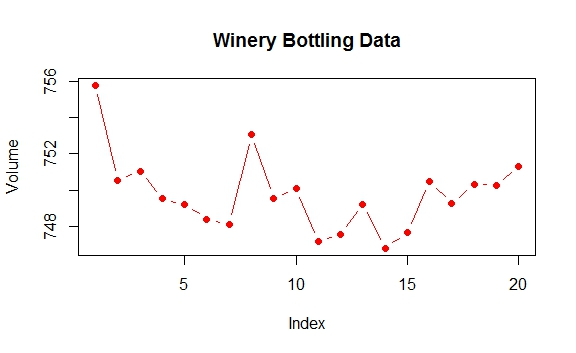
\includegraphics[width=0.9\linewidth]{./Winery}
\caption{}
\label{fig:Winery}
\end{figure}

%----------------------------------------------------------------------------------------------%
\newpage
\subsection{\texttt{ss.ca.z} Capability Indices}

Compute the Capability Indices of a process, Z (Sigma Score), $C_p$ and $C_{pk}$.
\begin{verbatim}
> ss.ca.cp(ss.data.ca$Volume,740, 760)
[1] 1.584136
> ss.ca.cpk(ss.data.ca$Volume,740, 760)
[1] 1.546513
> ss.ca.z(ss.data.ca$Volume,740,760)
[1] 3.139539
\end{verbatim}



\newpage
%--------------------------------------------------- %
\newpage
\subsection{Loss Fucntion Aanalysis}
The Taguchi Loss Function is graphical depiction of loss developed by the Japanese business statistician Genichi Taguchi to describe a phenomenon affecting the value of products produced by a company. Praised by Dr. W. Edwards Deming (the business guru of the 1980s American quality movement),[1] it made clear the concept that quality does not suddenly plummet when, for instance, a machinist exceeds a rigid blueprint tolerance. Instead "loss" in value progressively increases as variation increases from the intended condition. This was considered a breakthrough in describing quality, and helped fuel the continuous improvement movement that since has become known as lean manufacturing.

\begin{figure}[h!]
\centering
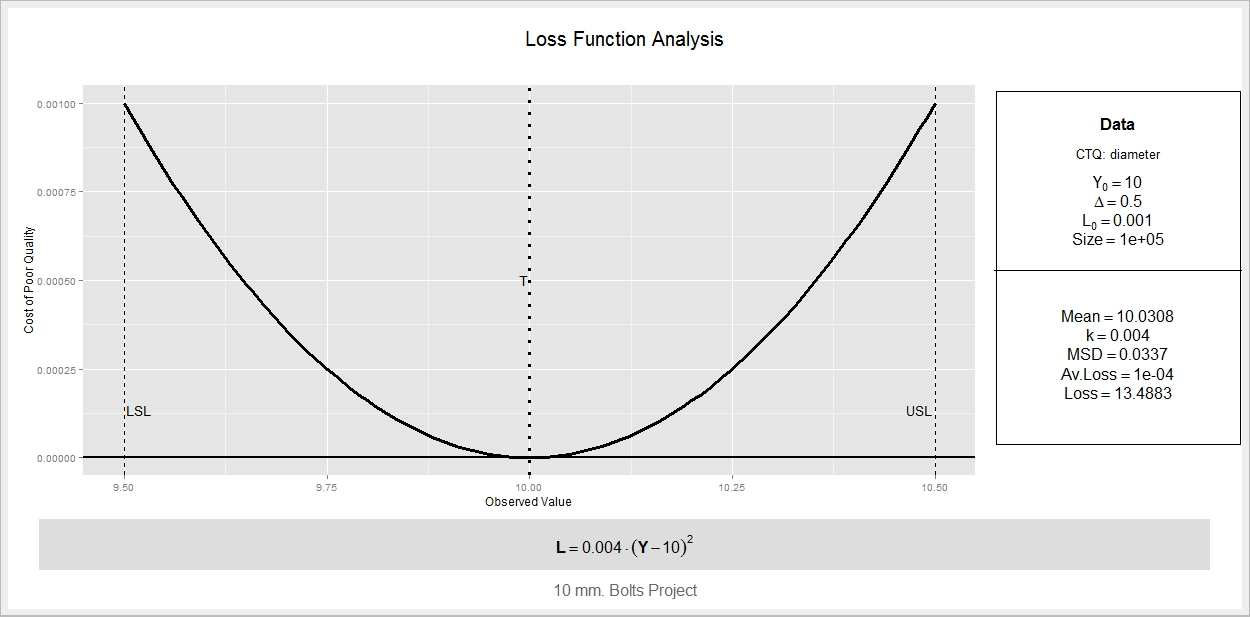
\includegraphics[width=0.7\linewidth]{images/LossFunctionAnalysis}
\caption{}
\label{fig:LossFunctionAnalysis}
\end{figure}
%------------------------------------------------------- %
\newpage
\section{Other R Packages}

\begin{enumerate}
\item mpci
\item mspc
\item qualityTools
\item spc
\item SixSigma with R (Emilio Cano)
\end{enumerate}


\newpage
\subsection{ \texttt{spc}: Statistical Process Control }

% Collection of Some Useful Functions

\begin{itemize}
\item Evaluation of control charts by means of the zero-state, steady-state ARL (Average Run Length) and RL quantiles. 

\item Setting up control charts for given in-control ARL. 

\item The control charts under consideration are one- and two-sided EWMA, CUSUM, and Shiryaev-Roberts schemes for monitoring the mean of normally distributed independent data. 

\item
ARL calculation of the same set of schemes under drift are added. 

\item Other charts and parameters are in preparation. 

\item Further SPC areas will be covered as well (sampling plans, capability indices ...)
\end{itemize}

%---------------------------------------------------------------------------------------------%

R package spc provides

\begin{verbatim}
xcusum.ad steady-state ARLs of CUSUM charts
xcusum.arl (zero-state) ARLs of CUSUM charts
xcusum.crit decision intervals of CUSUM charts
xewma.ad steady-state ARLs of EWMA charts
xewma.arl (zero-state) ARLs of EWMA charts
xewma.crit critical values of EWMA charts
\end{verbatim}




\end{document}
